\documentclass[11pt,a4paper]{article}
\usepackage[T1]{fontenc} \usepackage[utf8]{inputenc} \usepackage{lmodern} \usepackage{microtype} \usepackage{amsmath,amssymb,amsthm} \usepackage[margin=2.4cm]{geometry} \usepackage{titling} \usepackage{titlesec} \usepackage{tikz} \usepackage{pgfplots}
\pgfplotsset{compat=1.18} \pretitle{\begin{center}\vspace*{-1.2em}\Huge\bfseries\sffamily} \posttitle{\par\end{center}\vspace{0.4em}} \preauthor{\begin{center}\large\sffamily} \postauthor{\par\end{center}} \predate{} \postdate{}
\titleformat{\section}
{\LARGE\bfseries\sffamily}
{\thesection}
{0.75em}
{}
[\vspace{0.35em}{\titlerule[0.8pt]}] \titleformat{name=\section,numberless}
{\LARGE\bfseries\sffamily}
{}
{0em}
{}
[\vspace{0.35em}{\titlerule[0.8pt]}] \titleformat{\subsection}
{\Large\bfseries\sffamily}
{\thesubsection}
{0.65em}
{} \titleformat{\subsubsection}
{\large\bfseries\sffamily}
{\thesubsubsection}
{0.65em}
{}
\titlespacing*{\section}{0pt}{3.2ex plus 1ex minus .2ex}{1.6ex plus .2ex} \titlespacing*{\subsection}{0pt}{2.4ex plus .8ex minus .2ex}{1.1ex plus .2ex} \titlespacing*{\subsubsection}{0pt}{2ex plus .6ex minus .2ex}{1ex plus .2ex}
\theoremstyle{definition} \newtheorem{definition}{Definition} \theoremstyle{plain} \newtheorem{theorem}{Theorem}
\usepackage{hyperref}
\hypersetup{colorlinks=true, linkcolor=blue, urlcolor=blue, pdftitle={Calculus 1 Theory}, pdfauthor={Andrea}}
% Dedicated page for each part (vertically centred, book style)
\newcommand{\partpage}[2]{%
  \clearpage
  \thispagestyle{plain}%
  \phantomsection
  \addcontentsline{toc}{part}{Part #1 --- #2}%
  \null\vfill
  \begin{center}
    {\sffamily\Huge\bfseries Part #1\par}
    \vspace{4ex}
    \rule{0.55\textwidth}{1pt}\par
    \vspace{4ex}
    {\sffamily\LARGE\bfseries #2\par}
  \end{center}
  \vfill
}
\title{Calculus 1 Theory} \author{Andrea} \date{}
\begin{document} \maketitle
\tableofcontents
\partpage{I}{Preliminaries}
\clearpage
\section*{Introduction}
This document is a personal collection of the arguments and formulas I studied in Calculus~1. It is not a textbook and it does not aim at completeness. The goal is to keep in one place the theoretical material I want to be able to recall: definitions, main theorems, typical proof ideas, and the identities that come up when solving problems.
The notes follow the usual order of a first course in calculus of one real variable: the real line and limits, continuity, derivatives, applications of differentiation, integrals, and the fundamental theorems that connect them. Each later section should state the result clearly and record the argument at the level I used when studying it, without extra commentary.
When a formula or a theorem has a standard name, that name is kept so that it matches lectures and textbooks.
\clearpage
\section{Formalities: mathematical language}\label{sec:formalities}
Mathematics is written with a small number of precise words. The four that appear everywhere later are \emph{predicate}, \emph{statement}, \emph{universal implication} and \emph{theorem}.
\subsection{Predicate}
\begin{definition}[Predicate] A \emph{predicate} $P(x)$, $P(x,y)$, \ldots{} is an assertion that contains one or more free variables. On its own it is neither true nor false: it becomes true or false only after the variables are specified, or after they are bound by a quantifier. \end{definition}
Examples: \begin{align*} P(x) &\colon\quad x>0, \\ Q(x,y) &\colon\quad x^2+y^2=1, \\ R(n) &\colon\quad n\text{ is even}. \end{align*} $P(3)$ is true, $P(-1)$ is false. The expression $P(x)$ itself is not a statement.
The usual quantifiers turn a predicate into a statement:
\[\boxed{ \forall x\in A,\ P(x) \qquad\text{and}\qquad \exists x\in A,\ P(x). }\]
The first is true when $P(x)$ holds for every $x\in A$; the second when it holds for at least one $x\in A$.
\subsection{Statement}
\begin{definition}[Statement] A \emph{statement} is a declarative sentence that is either true or false, and not both. It has no free variables. \end{definition}
Examples of statements: $2+2=4$ (true); $\sqrt{2}$ is rational (false); $\forall x\in\mathbb{R},\ x^2\ge 0$ (true).
\subsection{Universal implication}
Most statements in calculus are not a single implication $P\Rightarrow Q$, but an implication that is required to hold for every object of a given type.
\begin{definition}[Universal implication] A \emph{universal implication} is a statement of the form
\[\boxed{ \forall x\in A,\quad P(x)\Rightarrow Q(x). }\]
$P(x)$ is the \emph{hypothesis} and $Q(x)$ is the \emph{conclusion}. It is read: for every $x\in A$, if $P(x)$ holds then $Q(x)$ holds. \end{definition}
The universal implication is true when every $x\in A$ that satisfies the hypothesis also satisfies the conclusion. It is false if and only if there exists a \emph{counterexample}: an element $x_0\in A$ such that $P(x_0)$ is true and $Q(x_0)$ is false.
To prove a universal implication one typically takes an arbitrary $x\in A$ with $P(x)$ and deduces $Q(x)$. To disprove it, it is enough to exhibit one counterexample.
The converse is
\[\boxed{ \forall x\in A,\quad Q(x)\Rightarrow P(x). }\]
It is a different statement; it may be true or false independently of the original implication. If both hold, one writes
\[\boxed{ \forall x\in A,\quad P(x)\Leftrightarrow Q(x). }\]
Then $P$ is a \emph{necessary and sufficient} condition for $Q$.
\subsection{Theorem}
\begin{definition}[Theorem] A \emph{theorem} is a statement that has been proved to be true. In these notes a theorem is almost always a universal implication, or a chain of such implications. \end{definition}
The same kind of true statement may be labelled in a weaker or stronger way according to its role: \begin{itemize}
\item a \emph{lemma} is a theorem used mainly as a step toward another result;
\item a \emph{proposition} is a theorem of intermediate importance;
\item a \emph{corollary} is a theorem that follows in a short way from a previous one. \end{itemize} A \emph{definition} is not a theorem: it introduces a name for an object or a property; it is neither proved nor disproved.
The standard pattern of a theorem in Calculus~1 is therefore: \begin{quote} \textbf{Theorem.} $\forall x\in A$, if $P(x)$ then $Q(x)$. \end{quote} followed by a \emph{proof}: a finite sequence of allowed deductions that starts from the hypothesis and ends at the conclusion.
\subsection{Law of contrapositives}
\begin{definition}[Law of contrapositives] The implication $P\Rightarrow Q$ is equivalent to its \emph{contrapositive} $\sim Q\Rightarrow \sim P$:
\[\boxed{ (P\Rightarrow Q)\quad\Leftrightarrow\quad (\sim Q\Rightarrow \sim P). }\]
The two statements are true together or false together. In particular they are not the converse $Q\Rightarrow P$. \end{definition}
For a universal implication the same law reads
\[\boxed{ \bigl(\forall x\in A,\ P(x)\Rightarrow Q(x)\bigr) \quad\Leftrightarrow\quad \bigl(\forall x\in A,\ \sim Q(x)\Rightarrow \sim P(x)\bigr). }\]
Therefore, to prove that $P(x)$ implies $Q(x)$ for every $x\in A$, it is enough to prove that whenever $Q(x)$ fails, $P(x)$ fails as well: take an arbitrary $x\in A$ with $\sim Q(x)$ and deduce $\sim P(x)$.
\subsection{Proof by contradiction}
\begin{definition}[Proof by contradiction] To prove a statement $R$ \emph{by contradiction}, assume $\sim R$ and deduce from that assumption a false statement (a contradiction, typically of the form $S\land\sim S$). Then $\sim R$ cannot hold, so $R$ is true. \end{definition}
When $R$ is a universal implication $\forall x\in A,\ P(x)\Rightarrow Q(x)$, a proof by contradiction proceeds as follows. Suppose the implication is false: there exists $x_0\in A$ such that $P(x_0)$ and $\sim Q(x_0)$. From these two assumptions one derives a contradiction. Hence no such $x_0$ exists, and the implication holds.
This is not the same argument as the law of contrapositives. The contrapositive proves $\sim Q\Rightarrow\sim P$ directly. A proof by contradiction assumes the negation of the claim one wants, and reaches an impossibility.
\clearpage
\section{Geometric progression}\label{sec:gprogress}
A \emph{geometric progression} (GP) is a sequence of real numbers
\[ (a_n)_{n\ge 0} \]
such that every term is obtained by multiplying the previous one by a fixed real number \(q\), called the \emph{ratio} of the progression.
\begin{definition}[Geometric progression] A sequence \((a_n)\) is a geometric progression of ratio \(q\) if
\[\boxed{ a_{n+1} = q\,a_n \qquad \text{for all } n\ge 0. }\]
\end{definition}
Starting from the initial term \(a_0\), the general term is
\[\boxed{ a_n = a_0\, q^n. }\]
\subsection{Geometric sum}
The basic geometric sum is
\[\boxed{ \sum_{k=0}^{n} q^k = \frac{1 - q^{\,n+1}}{1 - q} \qquad (q\neq 1). }\]
When \(q=1\), every term equals \(1\) and
\[ \sum_{k=0}^{n} 1 = n+1. \]
From this, the sum of the first \(n+1\) terms of a geometric progression is
\[ S_n = \sum_{k=0}^{n} a_k
= a_0 \sum_{k=0}^{n} q^k
= a_0\,\frac{1 - q^{\,n+1}}{1 - q}
\qquad (q\neq 1). \]
If \(q=1\), the progression is constant and
\[ S_n = (n+1)a_0. \]
\subsection{Infinite geometric series}
When \(|q|<1\), the geometric progression has a convergent infinite sum:
\[\boxed{ \sum_{n=0}^{\infty} a_n = \frac{a_0}{1-q}. }\]
If \(|q|\ge 1\), the infinite series diverges.
\subsection*{Examples}
\begin{equation*} \begin{aligned} a_n &= 3\cdot 2^n &&\text{GP with } a_0=3,\ q=2\\ a_n &= 5\left(\tfrac12\right)^n &&\text{GP with } a_0=5,\ q=\tfrac12 \end{aligned} \end{equation*}
\clearpage
\section{Binomial coefficients and Newton's formula}\label{sec:binomial}
\subsection{Binomial coefficients}
For every pair of integers $n\ge 0$ and $0\le k\le n$, the \emph{binomial coefficient} $\binom{n}{k}$ counts the number of ways to choose $k$ elements from a set of $n$ elements. It is defined by
\[\boxed{ \binom{n}{k} = \frac{n!}{k!\,(n-k)!}. }\]
The binomial coefficients satisfy the symmetry identity
\[\boxed{ \binom{n}{k} = \binom{n}{n-k}, }\]
and the recurrence relation
\[\boxed{ \binom{n}{k} = \binom{n-1}{k} + \binom{n-1}{k-1}, }\]
which is the rule that generates Pascal's triangle.
\subsection{Newton's binomial formula}
For every real numbers $x,y$ and every integer $n\ge 0$, the expansion of $(x+y)^n$ is given by the \emph{binomial formula}:
\[\boxed{ (x+y)^n = \sum_{k=0}^{n} \binom{n}{k}\, x^{n-k} y^{k}. }\]
Each term corresponds to choosing $k$ factors $y$ and $n-k$ factors $x$ in the product $(x+y)(x+y)\cdots(x+y)$ repeated $n$ times.
\subsection{Special cases}
Setting $x=1$ gives the identity
\[ (1+y)^n = \sum_{k=0}^{n} \binom{n}{k}\, y^{k}. \]
Setting $y=1$ gives
\[ (x+1)^n = \sum_{k=0}^{n} \binom{n}{k}\, x^{n-k}. \]
Setting $x=y=1$ yields the classical sum of the $n$-th row of Pascal's triangle:
\[ 2^n = \sum_{k=0}^{n} \binom{n}{k}. \]
\clearpage
\section{Fields and ordered fields}\label{sec:fields}
\subsection{Fields}
A \emph{field} is a set $F$ equipped with two binary operations, addition and multiplication, satisfying the axioms listed below. The elements of $F$ are called \emph{numbers}. The operations are written $x+y$ and $xy$ (or $x\cdot y$).
\subsection{R1: Axioms for addition}
The addition operation $+$ satisfies the following properties for all $x,y,z\in F$:
\begin{itemize}
\item \textbf{(R1.1) Commutativity:} $x+y = y+x$.
\item \textbf{(R1.2) Associativity:} $(x+y)+z = x+(y+z)$.
\item \textbf{(R1.3) Additive identity:} there exists an element $0\in F$
such that $x+0 = x$ for all $x\in F$.
\item \textbf{(R1.4) Additive inverse:} for every $x\in F$ there exists an
element $-x\in F$ such that $x+(-x)=0$. \end{itemize}
The element $0$ is called the \emph{additive identity}, and $-x$ is the \emph{additive inverse} of $x$.
\subsection{R2: Axioms for multiplication}
The multiplication operation $\cdot$ satisfies the following properties for all $x,y,z\in F$:
\begin{itemize}
\item \textbf{(R2.1) Commutativity:} $xy = yx$.
\item \textbf{(R2.2) Associativity:} $(xy)z = x(yz)$.
\item \textbf{(R2.3) Multiplicative identity:} there exists an element
$1\in F$, $1\neq 0$, such that $x\cdot 1 = x$ for all $x\in F$.
\item \textbf{(R2.4) Multiplicative inverse:} for every $x\in F$ with
$x\neq 0$ there exists an element $x^{-1}\in F$ such that
$x\cdot x^{-1} = 1$. \end{itemize}
The element $1$ is called the \emph{multiplicative identity}, and $x^{-1}$ is the \emph{multiplicative inverse} of $x$.
\subsection{Distributive law}
The two operations are connected by the distributive property:
\[ x(y+z) = xy + xz \qquad \text{for all } x,y,z\in F. \]
A set $F$ satisfying R1, R2, and the distributive law is called a \emph{field}.
\subsection{R3: Order relation}
An \emph{order relation} on $F$ is a binary relation $\le$ satisfying, for all $x,y,z\in F$:
\begin{itemize}
\item \textbf{(R3.1) Totality:} exactly one of the following holds:
$x<y$, $x=y$, or $x>y$.
\item \textbf{(R3.2) Transitivity:} if $x\le y$ and $y\le z$, then $x\le z$.
\item \textbf{(R3.3) Compatibility with addition:}
if $x\le y$, then $x+z \le y+z$.
\item \textbf{(R3.4) Compatibility with multiplication:}
if $0\le x$ and $0\le y$, then $0\le xy$. \end{itemize}
The relation $\le$ is called an \emph{order} on $F$.
\subsection{Ordered fields}
A field $F$ equipped with an order relation $\le$ satisfying R3 is called an \emph{ordered field}.
The standard examples of ordered fields are $\mathbb{Q}$ and $\mathbb{R}$.
\clearpage
\section{Supremum and Infimum}\label{sec:supremum}
Let $A\subseteq\mathbb{R}$ be a nonempty set. Since $\mathbb{R}$ is an ordered field, we can compare its elements and define upper and lower bounds.
\subsection{Upper bounds and supremum}
\begin{definition}[Upper bound] A real number $M$ is an \emph{upper bound} of $A$ if
\[ x \le M \qquad \text{for all } x\in A. \]
\end{definition}
\begin{definition}[Supremum] The \emph{supremum} (least upper bound) of $A$, denoted $\sup A$, is the smallest real number that is an upper bound of $A$.
A real number $s$ is $\sup A$ if and only if:
\begin{itemize}
\item every $x\in A$ satisfies $x\le s$;
\item for every $\varepsilon>0$ there exists $x\in A$ such that $x > s-\varepsilon$. \end{itemize}
\end{definition}
The second condition means that no number smaller than $s$ can be an upper bound.
\subsection{Lower bounds and infimum}
\begin{definition}[Lower bound] A real number $m$ is a \emph{lower bound} of $A$ if
\[ m \le x \qquad \text{for all } x\in A. \]
\end{definition}
\begin{definition}[Infimum] The \emph{infimum} (greatest lower bound) of $A$, denoted $\inf A$, is the largest real number that is a lower bound of $A$.
A real number $t$ is $\inf A$ if and only if:
\begin{itemize}
\item every $x\in A$ satisfies $t\le x$;
\item for every $\varepsilon>0$ there exists $x\in A$ such that $x < t+\varepsilon$. \end{itemize}
\end{definition}
\subsection{Existence in \texorpdfstring{$\mathbb{R}$}{R}}
Every nonempty set that is bounded above has a supremum, and every nonempty set that is bounded below has an infimum. This property is the \emph{completeness} of the real numbers.
\subsection*{Examples}
\begin{itemize}
\item For $A=(0,1)$, $\sup A=1$ and $\inf A=0$.
\item For $A=\{1/n : n\in\mathbb{N}\}$, $\sup A=1$ and $\inf A=0$.
\item For a finite set, $\sup A$ is its maximum and $\inf A$ is its minimum. \end{itemize}
\subsection{R4: Supremum property}
Let $X$ be an ordered field. We say that $X$ satisfies the \emph{supremum property} if:
\medskip
\textbf{(R4) Supremum property (continuity axiom):} every nonempty subset $E\subseteq X$ that is a proper subset of $X$ and is bounded above admits a supremum in $X$.
\medskip
This property is also called the \emph{continuity axiom} of the ordered field.
\medskip
If $X$ satisfies (R4), then every nonempty subset $E\subseteq X$ that is bounded below admits an infimum in $X$.
Indeed, one may apply (R4) to the set of all lower bounds of $E$, or equivalently to the set $-E=\{-x : x\in E\}$, using the correspondence
\[ \inf E = -\sup(-E). \]
\medskip
The ordered field $\mathbb{Q}$ does \emph{not} satisfy (R4): there exist nonempty subsets of $\mathbb{Q}$ that are bounded above but do not have a supremum in $\mathbb{Q}$.
A classical example is
\[ E = \{\,q\in\mathbb{Q} : q^2 < 2\,\}, \]
which is bounded above in $\mathbb{Q}$ but has no least upper bound in $\mathbb{Q}$, since $\sqrt{2}\notin\mathbb{Q}$.
The ordered field $\mathbb{R}$ \emph{does} satisfy (R4): every nonempty subset of $\mathbb{R}$ that is bounded above has a supremum in $\mathbb{R}$, and every nonempty subset that is bounded below has an infimum in $\mathbb{R}$.
\subsection{Axiomatic definition of \texorpdfstring{$\mathbb{R}$}{R}}
A \emph{real number system} $\mathbb{R}$ can be defined axiomatically as a set equipped with two operations $+$ and $\cdot$ and an order relation $\le$ such that:
\begin{itemize}
\item $\mathbb{R}$ is a field: it satisfies R1 (axioms for addition), R2 (axioms for multiplication), and the distributive law;
\item $\mathbb{R}$ is an ordered field: it is equipped with an order relation $\le$ satisfying R3 (order axioms);
\item $\mathbb{R}$ satisfies R4: the supremum property (continuity axiom). \end{itemize}
Thus $\mathbb{R}$ is an \emph{ordered field with the supremum property}, and this completeness axiom distinguishes $\mathbb{R}$ from $\mathbb{Q}$.
\clearpage
\section{Triangle inequality}\label{sec:triangle}
In the ordered field $\mathbb{R}$, the absolute value of a real number $x$ is defined by
\[ |x| = \begin{cases} x, & x\ge 0,\\ -x, & x<0. \end{cases} \]
The absolute value measures the distance of $x$ from $0$ on the real line.
The fundamental estimate relating absolute values is the \emph{triangle inequality}.
\begin{theorem}[Triangle inequality]\label{thm:triangle-inequality} For all real numbers $x,y\in\mathbb{R}$,
\[\boxed{ |x+y| \le |x| + |y|. }\]
\end{theorem}
This inequality expresses that the distance from $0$ to $x+y$ is never greater than the sum of the distances from $0$ to $x$ and from $0$ to $y$.
\subsection{Reverse triangle inequality}
A direct consequence of the triangle inequality is the \emph{reverse triangle inequality}:
\[\boxed{ \bigl|\,|x| - |y|\,\bigr| \le |x-y|. }\]
It states that the difference between the lengths $|x|$ and $|y|$ cannot exceed the length of their difference.
\subsection{Geometric interpretation}
On the real line, $|x-y|$ represents the distance between $x$ and $y$.
The triangle inequality corresponds to the fact that in any triangle, the length of one side is at most the sum of the lengths of the other two.
\subsection*{Examples}
\begin{itemize}
\item $|3 + (-5)| = | -2 | = 2 \le |3| + | -5 | = 8$.
\item $|1.2 + 4.7| = 5.9 \le 1.2 + 4.7 = 5.9$ (equality case).
\item Reverse inequality: $\bigl|\,|7| - |2|\,\bigr| = 5 \le |7-2| = 5$. \end{itemize}
\clearpage
\section{Principle of mathematical induction}\label{sec:induction}
Many statements in calculus and discrete mathematics concern all integers greater than or equal to a fixed starting point. The \emph{principle of mathematical induction} is the fundamental method used to prove such statements.
\begin{definition}[Principle of induction] Let $P(n)$ be a statement depending on an integer $n\ge n_0$.
We say that $P(n)$ holds for all integers $n\ge n_0$ if the following two conditions are satisfied:
\begin{itemize}
\item \textbf{(Base step)} The statement $P(n_0)$ is true.
\item \textbf{(Inductive step)} For every integer $k\ge n_0$,
if $P(k)$ is true, then $P(k+1)$ is true. \end{itemize}
Under these two assumptions, $P(n)$ is true for all integers $n\ge n_0$. \end{definition}
The base step verifies the statement at the starting point.
The inductive step shows that the truth of $P(k)$ forces the truth of $P(k+1)$, creating a chain of implications:
\[ P(n_0) \Rightarrow P(n_0+1) \Rightarrow P(n_0+2) \Rightarrow \cdots \]
\subsection{Strong induction}
A useful variant is \emph{strong induction}.
It states that $P(n)$ holds for all $n\ge n_0$ if:
\begin{itemize}
\item $P(n_0)$ is true;
\item for every $k\ge n_0$,
if $P(n_0), P(n_0+1), \ldots, P(k)$ are all true, then $P(k+1)$ is true. \end{itemize}
Strong induction is equivalent to ordinary induction, but often simplifies proofs where the inductive step depends on several previous cases.
\subsection*{Example}
To prove that
\[ \sum_{k=1}^{n} k = \frac{n(n+1)}{2} \]
for all integers $n\ge 1$:
\begin{itemize}
\item Base step: for $n=1$, both sides equal $1$.
\item Inductive step: assume the formula holds for $n=k$. Then
\[
\sum_{i=1}^{k+1} i
= \left(\sum_{i=1}^{k} i\right) + (k+1)
= \frac{k(k+1)}{2} + (k+1)
= \frac{(k+1)(k+2)}{2},
\]
which is the formula for $n=k+1$. \end{itemize}
Thus the identity holds for all $n\ge 1$ by induction.
\clearpage
\section{Complex numbers}\label{sec:complex}
Real numbers are not sufficient to solve all algebraic equations.
For example, the equation
\[ x^2 + 1 = 0 \]
has no solution in $\mathbb{R}$, since no real number has square $-1$.
To overcome this limitation, one introduces a new number $i$ satisfying
\[ i^2 = -1, \]
and defines the \emph{complex numbers} as all expressions of the form
\[ z = x + iy, \qquad x,y\in\mathbb{R}. \]
The set of complex numbers is denoted by $\mathbb{C}$.
Every complex number has a \emph{real part} $\Re(z)=x$ and an \emph{imaginary part} $\Im(z)=y$.
\subsection{Modulus and argument}
For a complex number $z=x+iy$, its \emph{modulus} is
\[ |z| = \sqrt{x^2 + y^2}, \]
and its \emph{argument} is the angle $\theta$ (with $\theta\in\mathbb{R}$) such that
\[ \cos\theta = \frac{x}{|z|}, \qquad \sin\theta = \frac{y}{|z|}. \]
The modulus represents the distance of $z$ from the origin in the complex plane, and the argument represents the direction of $z$.
\subsection{Trigonometric form}
Every nonzero complex number $z=x+iy$ can be written in \emph{trigonometric form}:
\[ z = |z|\bigl(\cos\theta + i\sin\theta\bigr), \]
where $|z|$ is the modulus and $\theta$ is the argument of $z$.
This representation is fundamental for multiplication, division, powers, and roots of complex numbers.
\subsection*{Examples}
\begin{itemize}
\item $z = 3 + 3i$ has $|z| = 3\sqrt{2}$ and $\theta = \pi/4$, so
\[
z = 3\sqrt{2}\left(\cos\frac{\pi}{4} + i\sin\frac{\pi}{4}\right).
\]
\item $z = -2i$ has $|z| = 2$ and $\theta = -\frac{\pi}{2}$. \end{itemize}
\subsection{De Moivre's formula}
For every complex number written in trigonometric form
\[ z = |z|\bigl(\cos\theta + i\sin\theta\bigr), \]
and for every integer $n\ge 1$, the powers of $z$ are given by \emph{De Moivre's formula}:
\[\boxed{ z^n = |z|^n\bigl(\cos(n\theta) + i\sin(n\theta)\bigr). }\]
This identity shows that raising a complex number to a power multiplies its argument by $n$ and raises its modulus to the $n$-th power.
\subsection{Roots}
De Moivre's formula also provides the $n$-th roots of a nonzero complex number.
If
\[ z = |z|\bigl(\cos\theta + i\sin\theta\bigr), \]
then the $n$ distinct $n$-th roots of $z$ are
\[ \sqrt[n]{z}_k = |z|^{1/n}\bigl(\cos\frac{\theta + 2k\pi}{n}
+ i\sin\frac{\theta + 2k\pi}{n}\bigr), \qquad k=0,1,\ldots,n-1. \]
Each root corresponds to dividing the argument by $n$ and adding the full rotations $\frac{2k\pi}{n}$.
\subsection*{Examples}
\begin{itemize}
\item For $z = \cos\theta + i\sin\theta$,
\[
z^5 = \cos(5\theta) + i\sin(5\theta).
\]
\item The cube roots of $1$ are
\[
\cos\frac{2k\pi}{3} + i\sin\frac{2k\pi}{3},
\qquad k=0,1,2.
\]
\end{itemize}
\subsection{n-th roots of a complex number}
Let $z$ be a nonzero complex number written in trigonometric form
\[ z = |z|\bigl(\cos\theta + i\sin\theta\bigr). \]
We want to determine all complex numbers $w$ such that $w^n = z$, where $n\ge 1$ is an integer.
A complex number $w$ is an $n$-th root of $z$ if and only if it has modulus
\[ |w| = |z|^{1/n} \]
and argument
\[ \arg(w) = \frac{\theta + 2k\pi}{n}, \qquad k = 0,1,\ldots,n-1. \]
Thus the $n$ distinct $n$-th roots of $z$ are
\[ w_k = |z|^{1/n}
\left(
\cos\frac{\theta + 2k\pi}{n}
+ i\sin\frac{\theta + 2k\pi}{n}
\right), \qquad k=0,1,\ldots,n-1. \]
These roots are equally spaced on the circle of radius $|z|^{1/n}$ in the complex plane, forming a regular $n$-gon centered at the origin.
\subsection*{Example}
The fourth roots of $1$ are
\[ \cos\frac{2k\pi}{4} + i\sin\frac{2k\pi}{4}, \qquad k=0,1,2,3, \]
that is,
\[ 1,\quad i,\quad -1,\quad -i. \]
\subsection{Fundamental theorem of algebra}
Complex numbers allow us to solve all polynomial equations.
In contrast, the real numbers are not sufficient: for example, the equation
\[ x^2 + 1 = 0 \]
has no real solution.
The introduction of the complex number $i$ with $i^2 = -1$ makes it possible to solve every polynomial equation of positive degree.
\begin{theorem}[Fundamental theorem of algebra]\label{thm:fundamental-algebra} Every nonconstant polynomial with complex coefficients has at least one complex root. \end{theorem}
Equivalently, if
\[ p(z) = a_n z^n + a_{n-1} z^{n-1} + \cdots + a_1 z + a_0, \qquad a_n \neq 0, \]
is a polynomial of degree $n\ge 1$, then there exists $z_0 \in \mathbb{C}$ such that $p(z_0)=0$.
\subsection*{Consequences}
The theorem implies several fundamental facts:
\begin{itemize}
\item Every polynomial of degree $n$ has exactly $n$ complex roots, counted with multiplicity.
\item Every polynomial can be factored completely over $\mathbb{C}$:
\[
p(z) = a_n (z - z_1)(z - z_2)\cdots(z - z_n).
\]
\item The field $\mathbb{C}$ is \emph{algebraically closed}: all algebraic equations can be solved within $\mathbb{C}$. \end{itemize}
\subsection*{Examples}
\begin{itemize}
\item The polynomial $z^2 + 1$ has the roots $i$ and $-i$.
\item The polynomial $z^3 - 1$ has the three roots
\[
1,\qquad
\cos\frac{2\pi}{3} + i\sin\frac{2\pi}{3},\qquad
\cos\frac{4\pi}{3} + i\sin\frac{4\pi}{3}.
\]
\end{itemize}
\partpage{II}{Calculus}
\clearpage
\section{Functions of one variable}\label{sec:functions}
A \emph{function} is a fundamental object in calculus. It assigns to each real number in a given set exactly one real number. Functions describe how quantities depend on one another and are represented geometrically in the Cartesian plane.
\subsection{Definition of a function}
\begin{definition}[Function] Let $A,B\subseteq\mathbb{R}$.
A \emph{function} is a rule
\[ f : A \to B \]
that assigns to every $x\in A$ a unique real number $f(x)\in B$.
The set $A$ is the \emph{domain} of $f$, the set $B$ is the \emph{codomain}, and the value $f(x)$ is the \emph{image} of $x$. \end{definition}
Thus a function is a special kind of relation: every input has exactly one output.
The collection of all pairs $(x,f(x))$ is the \emph{graph} of $f$:
\[ \operatorname{graph}(f)=\{(x,f(x)) : x\in A\}\subseteq\mathbb{R}^2. \]
\subsection{The Cartesian plane}
The \emph{Cartesian plane}, introduced by René Descartes, is the set of all ordered pairs of real numbers:
\[ \mathbb{R}^2 = \{(x,y) : x,y\in\mathbb{R}\}. \]
It is built from two perpendicular axes: \begin{itemize}
\item the horizontal axis (the $x$-axis), representing the input variable;
\item the vertical axis (the $y$-axis), representing the output variable. \end{itemize}
The axes intersect at the \emph{origin} $(0,0)$.
Every point $(x,y)$ in the plane corresponds to a unique pair of real numbers.
\subsection{Graph of a function}
The graph of a function $f$ is the set of points $(x,f(x))$ in the Cartesian plane.
It shows how the output varies as the input changes.
A curve in the plane represents a function if and only if no vertical line intersects it more than once.
This is the \emph{vertical line test}, expressing that each $x$ has exactly one $f(x)$.
\subsection*{Examples}
\begin{itemize}
\item $f(x)=x^2$: its graph is a parabola opening upward.
\item $f(x)=\frac{1}{x}$: its graph has two branches, one in each of the first and third quadrants.
\item $f(x)=\sin x$: its graph is a periodic wave oscillating between $-1$ and $1$. \end{itemize}
\subsection{Trigonometric functions}
The trigonometric functions $\sin$, $\cos$, and $\tan$ are defined using the geometry of the unit circle in the Cartesian plane.
For an angle $\theta$, measured from the positive $x$-axis, the point on the unit circle has coordinates
\[ (\cos\theta,\ \sin\theta). \]
The tangent function is defined as
\[ \tan\theta = \frac{\sin\theta}{\cos\theta}, \]
whenever $\cos\theta \neq 0$.
\subsection{Geometric representation}
\begin{center} 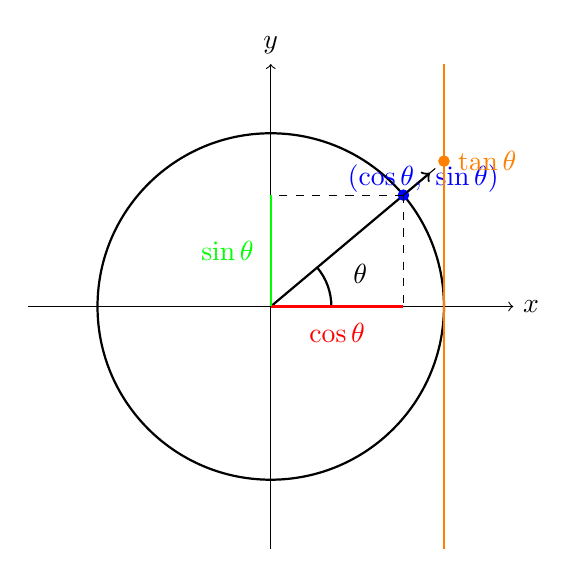
\begin{tikzpicture}[scale=2.2]
% Axes
\draw[->] (-1.4,0) -- (1.4,0) node[right] {$x$};
\draw[->] (0,-1.4) -- (0,1.4) node[above] {$y$};
% Unit circle
\draw[thick] (0,0) circle (1);
% Angle arc
\draw[thick] (0.35,0) arc (0:40:0.35);
% Angle label (near the origin)
\node at (20:0.55) {$\theta$};
% Ray forming the angle
\draw[thick,->] (0,0) -- (40:1.2);
% Point on the circle
\filldraw[blue] (40:1) circle (0.03);
\node[blue] at (40:1.15) {$(\cos\theta,\ \sin\theta)$};
% Cosine projection
\draw[dashed] (40:1) -- ({cos(40)},0);
\draw[thick,red] (0,0) -- ({cos(40)},0);
\node[red] at ({cos(40)/2},-0.15) {$\cos\theta$};
% Sine projection
\draw[dashed] (40:1) -- (0,{sin(40)});
\draw[thick,green] (0,0) -- (0,{sin(40)});
\node[green] at (-0.25,{sin(40)/2}) {$\sin\theta$};
% Tangent line
\draw[orange,thick] (1, -1.4) -- (1, 1.4);
\draw[dashed] (40:1) -- (1,{tan(40)});
\filldraw[orange] (1,{tan(40)}) circle (0.03);
\node[orange] at (1.25,{tan(40)}) {$\tan\theta$};
\end{tikzpicture} \end{center}
\subsection{Interpretation}
\begin{itemize}
\item $\cos\theta$ is the horizontal coordinate of the point on the unit circle.
\item $\sin\theta$ is the vertical coordinate.
\item $\tan\theta$ is the length of the segment where the ray at angle $\theta$
intersects the vertical line $x=1$. \end{itemize}
Thus the trigonometric functions arise naturally from the geometry of the unit circle.
\subsection{Inverse functions}
A function may admit an inverse only when it is \emph{injective}: different inputs must produce different outputs.
Formally, a function $f : A \to B$ is injective when
\[ f(x_1)=f(x_2) \;\Rightarrow\; x_1=x_2. \]
Injectivity ensures that every value in the image of $f$ corresponds to exactly one input.
In this case one can define the \emph{inverse function} $f^{-1}$, which reverses the action of $f$.
\begin{definition}[Inverse function] Let $f : A \to B$ be an injective function.
The \emph{inverse function} of $f$ is the map
\[ f^{-1} : f(A) \to A \]
satisfying
\[\boxed{ f^{-1}(f(x)) = x \qquad \text{for all } x\in A. }\]
\end{definition}
The graph of $f^{-1}$ is obtained by reflecting the graph of $f$ across the line $y=x$, called the \emph{bisector} of the first and third quadrants.
\subsection{Geometric representation}
\begin{center} 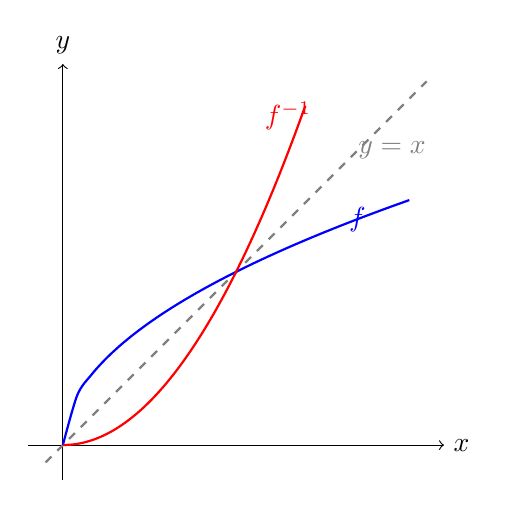
\begin{tikzpicture}[scale=2.2]
% Axes
\draw[->] (-0.2,0) -- (2.2,0) node[right] {$x$};
\draw[->] (0,-0.2) -- (0,2.2) node[above] {$y$};
% Bisector y = x
\draw[gray,thick,dashed] (-0.1,-0.1) -- (2.1,2.1);
\node[gray] at (1.9,1.7) {$y=x$};
% Function f(x) = sqrt(x)
\draw[blue,thick,domain=0:2,smooth,variable=\x]
plot ({\x},{sqrt(\x)});
\node[blue] at (1.7,1.3) {$f$};
% Inverse function f^{-1}(x) = x^2
\draw[red,thick,domain=0:1.4,smooth,variable=\x]
plot ({\x},{\x*\x});
\node[red] at (1.3,1.9) {$f^{-1}$};
\end{tikzpicture} \end{center}
The bisector $y=x$ shows that the inverse function is obtained by exchanging the roles of input and output: the graph of $f^{-1}$ is the reflection of the graph of $f$ across this line.
\clearpage
\section{Limits and continuity}\label{sec:limits}
Many concepts in calculus are based on the idea of approaching a value without necessarily reaching it.
The simplest objects that illustrate this behaviour are \emph{sequences} of real numbers.
They provide the first setting in which limits are defined and studied.
\subsection{Sequences}
A \emph{sequence} is an ordered list of real numbers
\[ (a_n)_{n\ge 0} = a_0, a_1, a_2, \ldots \]
indexed by the integers $n\ge 0$.
Formally, a sequence is a function
\[ a : \mathbb{N} \to \mathbb{R}, \qquad n \mapsto a_n, \]
where $\mathbb{N}$ denotes the set of non-negative integers.
The value $a_n$ is called the \emph{$n$-th term} of the sequence.
A sequence may be described by an explicit formula (for example $a_n = 1/n$) or by a recurrence relation (for example $a_{n+1} = q\,a_n$).
\subsection{Convergence of a sequence}
A sequence may approach a real number as $n$ becomes large.
This behaviour is captured by the notion of \emph{limit}.
\begin{definition}[Limit of a sequence] A sequence $(a_n)$ \emph{converges} to a real number $L$ if for every $\varepsilon > 0$ there exists an integer $N$ such that
\[ |a_n - L| < \varepsilon \qquad \text{for all } n \ge N. \]
In this case one writes
\[ \lim_{n\to\infty} a_n = L. \]
\end{definition}
If no such real number $L$ exists, the sequence is said to \emph{diverge}.
\subsection{Eventual behaviour of a sequence}
Many properties of sequences do not need to hold for every index.
It is often enough that they hold \emph{eventually}, that is, from some point onward.
\begin{definition}[Eventually] Let $(a_n)$ be a sequence of real numbers.
A property $P(n)$ is said to hold \emph{eventually} (or \emph{for all sufficiently large $n$}) if there exists an integer $N$ such that
\[ P(n) \qquad \text{holds for all } n \ge N. \]
\end{definition}
In other words, a sequence may fail to satisfy $P(n)$ for the first few terms, but as long as the property holds for all indices beyond some threshold $N$, it is considered to hold eventually.
This notion is fundamental in limit theory, where statements about $a_n$ approaching a value concern the behaviour of the sequence for large $n$, not its initial terms.
\subsection{Types of behaviour of a sequence}
A sequence may exhibit different kinds of behaviour as the index $n$ becomes large.
The standard distinction is the following.
\subsubsection*{Convergent sequences}
A sequence $(a_n)$ is \emph{convergent} if it has a real limit, that is, if there exists $L\in\mathbb{R}$ such that
\[ \lim_{n\to\infty} a_n = L. \]
\subsubsection*{Sequences divergent to infinity}
A sequence is said to \emph{diverge to $+\infty$} if its terms grow without bound, meaning that for every $M\in\mathbb{R}$ there exists $N$ such that
\[ a_n > M \qquad \text{for all } n \ge N. \]
Similarly, it \emph{diverges to $-\infty$} if for every $M\in\mathbb{R}$ there exists $N$ such that
\[ a_n < M \qquad \text{for all } n \ge N. \]
In this sense, a ``divergent sequence'' is one whose terms tend to infinity in absolute value.
\subsubsection*{Sequences that are neither convergent nor divergent}
A sequence may fail to converge and also fail to diverge to $\pm\infty$.
Such sequences are described as \emph{neither convergent nor divergent}.
They may display oscillatory behaviour, irregular variation, or possess multiple accumulation points.
These sequences do not approach any single real value, nor do they grow without bound.
\subsection{Squeeze Theorem}
The Squeeze Theorem provides a useful criterion for determining the limit of a sequence by comparing it with two other sequences whose limits are known.
\begin{theorem}[Squeeze Theorem]\label{thm:squeeze} Let $(a_n)$, $(b_n)$, and $(c_n)$ be sequences of real numbers such that
\[ a_n \le b_n \le c_n \qquad \text{for all sufficiently large } n. \]
If
\[ \lim_{n\to\infty} a_n = L \qquad \text{and} \qquad \lim_{n\to\infty} c_n = L, \]
then the sequence $(b_n)$ also converges to $L$, that is,
\[ \lim_{n\to\infty} b_n = L. \]
\end{theorem}
The theorem states that if a sequence is eventually trapped between two convergent sequences sharing the same limit, then it must converge to that limit as well.
\subsection{The exponential limit and the number \texorpdfstring{$e$}{e}}
The number $e$ plays a central role in calculus and analysis.
It is defined through the behaviour of a specific sequence.
\begin{theorem}[Limit defining the number $e$]\label{thm:limit-e} The sequence
\[ a_n = \left(1+\frac{1}{n}\right)^n \]
is increasing and bounded above.
Therefore it is convergent, and its limit is denoted by $e$:
\[ \lim_{n\to\infty} \left(1+\frac{1}{n}\right)^n = e. \]
\end{theorem}
The number $e$ is thus characterized as the unique real value approached by the sequence $\left(1+\frac{1}{n}\right)^n$ as $n$ becomes large.
This limit provides the fundamental definition of the base of the natural logarithm.
\subsection{Asymptotic comparisons and estimates}
Asymptotic analysis studies the behaviour of sequences for large values of the index.
It provides tools to compare the growth of different sequences and to obtain useful approximations.
\subsection*{Asymptotic comparison}
Let $(a_n)$ and $(b_n)$ be sequences of real numbers.
We say that $a_n$ and $b_n$ have the same asymptotic behaviour if
\[ \lim_{n\to\infty} \frac{a_n}{b_n} = 1. \]
In this case we write
\[ a_n \sim b_n, \]
and say that $a_n$ is \emph{asymptotically equivalent} to $b_n$.
This relation expresses that the two sequences grow at the same rate, even if their initial terms may differ.
\subsection*{Asymptotic estimates}
A sequence $(a_n)$ is said to be \emph{of smaller order} than $(b_n)$ if
\[ \lim_{n\to\infty} \frac{a_n}{b_n} = 0, \]
and we write
\[ a_n = o(b_n). \]
This means that $a_n$ grows strictly slower than $b_n$.
Similarly, we say that $a_n$ is \emph{bounded in order} by $b_n$ if there exists a constant $C>0$ such that
\[ |a_n| \le C\,|b_n| \qquad \text{for all sufficiently large } n. \]
In this case we write
\[ a_n = O(b_n). \]
These notations allow us to express growth rates and approximations in a concise and effective way.
\subsection*{Asymptotic inequalities}
Asymptotic comparisons often rely on inequalities that hold eventually.
If for sufficiently large $n$ we have
\[ a_n \le b_n, \]
then the growth of $(a_n)$ is asymptotically controlled by that of $(b_n)$. Such inequalities are frequently used to establish limits or to derive asymptotic estimates.
\subsection{Ratio Test}
The ratio test provides a useful criterion for determining whether a sequence diverges to $+\infty$ or converges to $0$, based on the behaviour of the ratio between consecutive terms.
\begin{theorem}[Ratio Test]\label{thm:ratio-test-limits} Let $(a_n)$ be a sequence of positive real numbers and suppose that the limit
\[ L = \lim_{n\to\infty} \frac{a_{n+1}}{a_n} \]
exists.
\begin{itemize}
\item If $L < 1$, then the sequence $(a_n)$ converges to $0$.
\item If $L > 1$, then the sequence $(a_n)$ diverges to $+\infty$.
\item If $L = 1$, the test is inconclusive: the sequence may converge, diverge,
or display irregular behaviour. \end{itemize} \end{theorem}
The ratio test compares the growth of consecutive terms.
If each term is eventually smaller than the previous one by a fixed proportion, the sequence must tend to zero.
If each term is eventually larger by a fixed proportion, the sequence grows without bound.
\subsection{Uniqueness of the limit}
The limit of a sequence, when it exists, is uniquely determined.
This fundamental property ensures that a sequence cannot converge to two different real numbers.
\begin{theorem}[Uniqueness of the limit]\label{thm:uniqueness-limit} Let $(a_n)$ be a sequence of real numbers.
If $(a_n)$ converges to $L$ and also converges to $M$, then
\[ L = M. \]
\end{theorem}
In other words, a convergent sequence cannot have two distinct limits.
The eventual behaviour of the sequence determines a single real value, which is its unique limit.
\subsection{Limits of functions}
From sequences we pass to functions: the \emph{limit of a function} at a point $x_0$ describes the behaviour of $f(x)$ as $x$ approaches $x_0$ without necessarily reaching it. The precise formulation is obtained through the one-sided limits introduced next.
\subsection{Right and left limits of a function}
When studying the behaviour of a function near a point, it is often necessary to distinguish between approaching the point from the left or from the right.
\begin{definition}[Right limit] Let $f$ be a real function and let $x_0$ be a point in its domain.
The \emph{right limit} of $f$ at $x_0$ is the value $L$ such that
\[ \lim_{x \to x_0^+} f(x) = L, \]
meaning that $f(x)$ approaches $L$ as $x$ approaches $x_0$ from values greater than $x_0$. \end{definition}
\begin{definition}[Left limit] The \emph{left limit} of $f$ at $x_0$ is the value $M$ such that
\[ \lim_{x \to x_0^-} f(x) = M, \]
meaning that $f(x)$ approaches $M$ as $x$ approaches $x_0$ from values smaller than $x_0$. \end{definition}
\subsection{Existence of the limit}
A function has a limit at a point if and only if both one-sided limits exist and are equal.
\begin{theorem}[Existence of the limit]\label{thm:existence-limit} Let $f$ be a real function and let $x_0$ be a point in its domain.
The limit
\[ \lim_{x \to x_0} f(x) \]
exists and equals $L$ if and only if
\[ \lim_{x \to x_0^-} f(x) = L \qquad \text{and} \qquad \lim_{x \to x_0^+} f(x) = L. \]
\end{theorem}
Thus, the behaviour of the function near $x_0$ is fully determined by its left-hand and right-hand limits.
If these two values coincide, the function has a well-defined limit at $x_0$.
\subsection{Jump discontinuity}
A function may fail to be continuous at a point because its left-hand and right-hand limits exist but are different.
This type of discontinuity is called a \emph{jump discontinuity}.
\begin{definition}[Jump discontinuity] Let $f$ be a real function and let $x_0$ be a point in its domain.
We say that $f$ has a \emph{jump discontinuity} at $x_0$ if the one-sided limits
\[ \lim_{x \to x_0^-} f(x) \qquad \text{and} \qquad \lim_{x \to x_0^+} f(x) \]
both exist as finite real numbers, but
\[ \lim_{x \to x_0^-} f(x) \ne \lim_{x \to x_0^+} f(x). \]
\end{definition}
In this case the function ``jumps'' from one value to another when crossing the point $x_0$.
The function cannot be continuous at $x_0$, since continuity requires the left-hand and right-hand limits to coincide and equal the value of the function.
\subsection{Neighbourhood of a point}
The behaviour of a function near a point is often described using the notion of a neighbourhood.
A neighbourhood specifies a small interval around a point, without necessarily including the point itself.
\begin{definition}[Neighbourhood] Let $x_0 \in \mathbb{R}$ and let $\delta > 0$.
The \emph{neighbourhood} of $x_0$ of radius $\delta$ is the interval
\[ (x_0 - \delta,\; x_0 + \delta). \]
It contains all real numbers whose distance from $x_0$ is less than $\delta$. \end{definition}
\begin{definition}[Punctured neighbourhood] The \emph{punctured neighbourhood} of $x_0$ of radius $\delta$ is the set
\[ (x_0 - \delta,\; x_0 + \delta) \setminus \{x_0\}. \]
It includes all points sufficiently close to $x_0$, but excludes $x_0$ itself. \end{definition}
Neighbourhoods and punctured neighbourhoods are used to describe limits and continuity, since limits concern the behaviour of a function near a point rather than at the point itself.
\subsection{Change of variable in limits}
When evaluating limits, it is often useful to replace the variable with another expression that approaches the same value.
The following theorem formalizes this idea.
\begin{theorem}[Change of variable in limits]\label{thm:change-variable-limits} Let $f$ be a real function and let $g$ be another function such that
\[ \lim_{x \to x_0} g(x) = L. \]
If the limit
\[ \lim_{y \to L} f(y) \]
exists and equals $M$, then the composite limit
\[ \lim_{x \to x_0} f(g(x)) \]
also exists and equals $M$. \end{theorem}
In other words, if $g(x)$ approaches $L$ as $x$ approaches $x_0$, and $f(y)$ approaches $M$ as $y$ approaches $L$, then the composition $f(g(x))$ approaches $M$ as $x$ approaches $x_0$.
The change of variable allows us to evaluate limits by substituting the inner expression with its limiting value.
\subsection{Continuity of elementary functions}
Elementary functions encountered in calculus possess strong continuity properties.
The following results summarize the fundamental facts.
\begin{definition}[Continuity of elementary functions] The basic elementary functions --- polynomials, rational functions (where defined), exponential and logarithmic functions, trigonometric and inverse trigonometric functions --- are continuous on every point of their domain. \end{definition}
\begin{definition}[Continuity preserved by algebraic operations] Let $f$ and $g$ be continuous at a point $x_0$.
Then the functions
\[ f+g,\qquad f-g,\qquad f\cdot g,\qquad \frac{f}{g}\ \text{(if } g(x_0)\ne 0) \]
are also continuous at $x_0$. \end{definition}
\begin{definition}[Continuity preserved by composition] If $f$ is continuous at $x_0$ and $g$ is continuous at $f(x_0)$, then the composition $g\circ f$ is continuous at $x_0$:
\[ \lim_{x\to x_0} g(f(x)) = g\bigl(\lim_{x\to x_0} f(x)\bigr). \]
\end{definition}
These properties ensure that any function built from elementary functions using algebraic operations and composition remains continuous on its domain.
\subsection{Fundamental limits}
Certain limits play a central role in calculus and appear frequently in the study of derivatives, continuity, and asymptotic behaviour.
These are known as \emph{fundamental limits}.
\begin{itemize}
\item \textbf{Exponential limit}
\[
\lim_{x \to 0} (1+x)^{1/x} = e.
\]
\item \textbf{Logarithmic limit}
\[
\lim_{x \to 0} \frac{\ln(1+x)}{x} = 1.
\]
\item \textbf{Trigonometric limits}
\[
\lim_{x \to 0} \frac{\sin x}{x} = 1,
\qquad
\lim_{x \to 0} \frac{1 - \cos x}{x^2} = \frac{1}{2}.
\]
\item \textbf{Exponential growth limit}
\[
\lim_{x \to 0} \frac{e^x - 1}{x} = 1.
\]
\item \textbf{Power limit}
\[
\lim_{x \to 0} \frac{x^n}{x} = 0 \qquad \text{for every } n>1.
\]
\end{itemize}
These limits are used to compute derivatives of elementary functions and to establish many foundational results in analysis.
They also serve as reference points for approximations and asymptotic estimates.
\subsection{Theorem of the zeros}
A continuous function on an interval cannot change sign without crossing the value zero.
This fundamental result is known as the \emph{Theorem of the zeros}.
\begin{theorem}[Theorem of the zeros]\label{thm:zeros} Let $f$ be a real function that is continuous on the closed interval $[a,b]$. If
\[ f(a)\cdot f(b) < 0, \]
that is, if $f(a)$ and $f(b)$ have opposite signs, then there exists at least one point $c \in (a,b)$ such that
\[ f(c) = 0. \]
\end{theorem}
In other words, a continuous function that takes positive values at one endpoint of an interval and negative values at the other must vanish somewhere inside the interval.
The function cannot ``jump over'' the value zero without violating continuity.
\subsection{Weierstrass Theorem}
A continuous function defined on a closed and bounded interval always reaches its largest and smallest values.
This fundamental result is known as the \emph{Weierstrass Theorem}.
\begin{theorem}[Weierstrass Theorem]\label{thm:weierstrass} Let $f$ be a real function that is continuous on the closed interval $[a,b]$. Then $f$ is bounded on $[a,b]$, and there exist points
\[ x_{\min},\; x_{\max} \in [a,b] \]
such that
\[ f(x_{\min}) = \min_{x \in [a,b]} f(x), \qquad f(x_{\max}) = \max_{x \in [a,b]} f(x). \]
\end{theorem}
In other words, a continuous function on a closed interval cannot ``escape'' to infinity and cannot approach its extrema without attaining them.
The compactness of the interval ensures both boundedness and the existence of maximum and minimum values.
\subsection{Intermediate Value Theorem}
A continuous function on an interval cannot ``skip'' values.
If it takes two different values at the endpoints of an interval, then it must take every value in between.
This fundamental result is known as the \emph{Intermediate Value Theorem}.
\begin{theorem}[Intermediate Value Theorem]\label{thm:intermediate-value} Let $f$ be a real function that is continuous on the closed interval $[a,b]$. Let $L$ be any real number between $f(a)$ and $f(b)$, that is,
\[ f(a) < L < f(b) \quad \text{or} \quad f(b) < L < f(a). \]
Then there exists at least one point $c \in (a,b)$ such that
\[ f(c) = L. \]
\end{theorem}
In other words, a continuous function on an interval takes all intermediate values between its values at the endpoints.
The function cannot jump over any value without violating continuity.
\subsection{Existence and uniqueness of the \texorpdfstring{$n$}{n}th root}
The $n$th root of a positive real number is well defined and unique.
This fundamental property ensures that the equation $x^n = y$ has exactly one positive solution.
\begin{theorem}[Existence and uniqueness of the $n$th root]\label{thm:nth-root} For every real number $y>0$ and every integer $n \ge 1$, there exists one and only one real number $x>0$ such that
\[ x^n = y. \]
This number is called the $n$th root of $y$ and is denoted by $\sqrt[n]{y}$. \end{theorem}
In other words, the function $x \mapsto x^n$ is continuous and strictly increasing on $(0,+\infty)$, and therefore it admits a unique inverse on this interval.
This inverse function assigns to each positive $y$ its unique positive $n$th root.
\subsection{Monotonicity theorem for functions}
A monotone function on an interval has well-defined one-sided limits at every point of the interval.
Inside the interval these limits are finite, while at the endpoints they may be finite or infinite.
\begin{theorem}[Monotonicity theorem]\label{thm:monotonicity} Let $f$ be a real function that is monotone (increasing or decreasing) on the interval $[a,b]$.
\begin{itemize}
\item For every point $x_0 \in (a,b)$, both one-sided limits
\[
\lim_{x \to x_0^-} f(x)
\qquad\text{and}\qquad
\lim_{x \to x_0^+} f(x)
\]
exist and are finite.
\item At the left endpoint $a$, the right-hand limit
\[
\lim_{x \to a^+} f(x)
\]
exists and may be finite or $+\infty$ or $-\infty$.
\item At the right endpoint $b$, the left-hand limit
\[
\lim_{x \to b^-} f(x)
\]
exists and may be finite or $+\infty$ or $-\infty$. \end{itemize} \end{theorem}
In other words, monotonicity ensures that the function has a well-defined behaviour near every point of the interval:
inside the interval the function cannot oscillate, and at the endpoints it may diverge but never oscillate.
\clearpage
\section{Differential Calculus}\label{sec:derivatives}
Differential calculus studies how functions change and how their behaviour can be described locally.
Its central concept is the derivative, which measures the instantaneous rate of variation of a function with respect to its variable.
Through limits, we develop tools to understand linear approximations, tangent lines, and the sensitivity of functions to small changes in input.
This section introduces the derivative, explores its fundamental properties, and presents the main rules of differentiation.
We also examine differentiability, the relationship between continuity and derivatives, and the applications of derivatives to monotonicity, extrema, and the qualitative analysis of functions.
\subsection{Derivative of a function}
Let $f$ be a real function defined on a subset of $\mathbb{R}$.
As stated earlier, a function is a rule $f:A\to B$ that assigns to every $x\in A$ a unique real number $f(x)\in B$.
The derivative describes how $f(x)$ changes when $x$ varies.
\begin{definition}[Derivative] The \emph{derivative} of $f$ at a point $x_0$ is the limit
\[\boxed{ f'(x_0) = \lim_{h\to 0} \frac{f(x_0+h)-f(x_0)}{h}, }\]
if this limit exists. \end{definition}
The quotient
\[ \frac{f(x_0+h)-f(x_0)}{h} \]
is the slope of the secant line through the points $(x_0,f(x_0))$ and $(x_0+h,f(x_0+h))$.
The derivative $f'(x_0)$ is the slope of the tangent line obtained as the limit of these secant slopes.
\subsection{Slope and tangent line}
The tangent line to the graph of $f$ at $x_0$ is the line
\[ y = f(x_0) + f'(x_0)(x - x_0). \]
\begin{itemize}
\item If $f'(x_0)>0$, the graph is increasing at $x_0$.
\item If $f'(x_0)<0$, the graph is decreasing at $x_0$.
\item If $f'(x_0)=0$, the tangent line is horizontal. \end{itemize}
\subsection*{Angle of inclination}
Every nonvertical line has an angle of inclination $\theta$ with the positive $x$-axis.
The slope $m$ and the angle $\theta$ are related by
\[ m = \tan\theta. \]
Therefore, if the tangent line at $x_0$ makes an angle $\theta$ with the $x$-axis, then
\[ f'(x_0) = \tan\theta. \]
A large absolute value of $f'(x_0)$ corresponds to a steep tangent line.
If the tangent line is vertical, the angle is $\theta=\frac{\pi}{2}$ and the slope is undefined: the derivative does not exist at that point.
\subsection*{Elementary derivatives}
The following table collects the basic derivatives of the standard elementary functions.
Each formula holds for every $x$ in the domain where the expression is defined.
\begin{center} \renewcommand{\arraystretch}{1.4} \begin{tabular}{|c|c|} \hline \textbf{Function $f(x)$} & \textbf{Derivative $f'(x)$} \\ \hline $c$ (constant) & $0$ \\ \hline $x$ & $1$ \\ \hline $x^n$ (for $n\in\mathbb{Z}$) & $n x^{\,n-1}$ \\ \hline $\sqrt{x}$ & $\dfrac{1}{2\sqrt{x}}$ \\ \hline $\dfrac{1}{x}$ & $-\dfrac{1}{x^2}$ \\ \hline $\sin x$ & $\cos x$ \\ \hline $\cos x$ & $-\sin x$ \\ \hline $\tan x$ & $\sec^2 x$ \\ \hline $\cot x$ & $-\csc^2 x$ \\ \hline $\sec x$ & $\sec x \tan x$ \\ \hline $\csc x$ & $-\csc x \cot x$ \\ \hline $e^x$ & $e^x$ \\ \hline $a^x$ ($a>0$) & $a^x \ln a$ \\ \hline $\ln x$ & $\dfrac{1}{x}$ \\ \hline $\log_a x$ ($a>0$) & $\dfrac{1}{x \ln a}$ \\ \hline \end{tabular} \end{center}
\subsection{Corner points, cusps, and inflection points}
The derivative describes the local behaviour of the graph of a function.
Certain characteristic points occur when the derivative fails to exist or when the curvature of the graph changes.
\subsection*{Corner point}
A point $x_0$ is a \emph{corner point} of the graph of $f$ if the one-sided derivatives
\[ f'_-(x_0) = \lim_{h\to 0^-} \frac{f(x_0+h)-f(x_0)}{h}, \qquad f'_+(x_0) = \lim_{h\to 0^+} \frac{f(x_0+h)-f(x_0)}{h} \]
both exist but are different:
\[ f'_-(x_0) \neq f'_+(x_0). \]
The tangent line has a sudden change of slope, producing a sharp angle on the graph.
\subsection*{Cusp}
A point $x_0$ is a \emph{cusp} if the one-sided derivatives diverge with opposite signs:
\[ f'_-(x_0) = -\infty, \qquad f'_+(x_0) = +\infty, \]
or vice versa.
The graph approaches a vertical tangent from both sides, but with incompatible directions, creating a pointed tip.
\subsection*{Inflection point}
A point where the concavity changes sign is called an \emph{inflection point}. The systematic study of inflection points -- the criterion based on the second derivative and the behaviour of the tangent line -- is developed at the end of this section.
\subsection*{Summary}
\begin{itemize}
\item Corner point: one-sided derivatives exist but are different.
\item Cusp: one-sided derivatives diverge with opposite signs.
\item Inflection point: concavity changes sign; the tangent line exists. \end{itemize}
\subsection*{Continuity and differentiability}
Differentiability is a stronger property than continuity.
A function may be continuous without being differentiable, but every differentiable function is necessarily continuous.
\begin{theorem}[Differentiability implies continuity]\label{thm:differentiability-continuity} Let $f$ be a function defined on an interval and let $x_0$ be a point in its domain.
If $f$ is differentiable at $x_0$, then $f$ is continuous at $x_0$. \end{theorem}
\subsection*{Continuity without differentiability}
The converse is false: continuity does not imply differentiability.
A function may be continuous at a point but fail to have a derivative there.
Typical examples include: \begin{itemize}
\item corner points (e.g.\ $f(x)=|x|$ at $x=0$),
\item cusps (e.g.\ $f(x)=x^{2/3}$ at $x=0$),
\item vertical tangents (e.g.\ $f(x)=\sqrt[3]{x}$ at $x=0$). \end{itemize}
\subsection*{Summary}
\begin{itemize}
\item Differentiability $\Rightarrow$ continuity.
\item Continuity $\not\Rightarrow$ differentiability.
\item Non-differentiability may occur at corners, cusps, or vertical tangents. \end{itemize}
\subsection{Derivative of an inverse function}
Let $f$ be a real function defined on an interval.
When $f$ is strictly monotonic, it is invertible, and its inverse function $f^{-1}$ is also defined on an interval.
The derivative of the inverse is determined by the derivative of $f$.
\begin{theorem}[Derivative of the inverse function]\label{thm:derivative-inverse} Let $f$ be a continuous and strictly monotonic function on an interval, and assume that $f$ is differentiable at a point $x_0$ with
\[ f'(x_0) \neq 0. \]
Then the inverse function $f^{-1}$ is differentiable at $y_0 = f(x_0)$, and its derivative is
\[ (f^{-1})'(y_0) = \frac{1}{f'(x_0)}. \]
Equivalently, for every $x$ in the domain of $f$,
\[ (f^{-1})'(f(x)) = \frac{1}{f'(x)}. \]
\end{theorem}
\subsection*{Interpretation}
The derivative of the inverse function is the reciprocal of the derivative of the original function.
Geometrically, the graph of $f^{-1}$ is the reflection of the graph of $f$ across the line $y=x$, and the slope transforms by inversion:
\[ m_{f^{-1}} = \frac{1}{m_f}. \]
\subsection*{Example}
For $f(x)=e^x$, the inverse is $f^{-1}(y)=\ln y$.
Since $f'(x)=e^x$, we obtain
\[ (\ln y)' = \frac{1}{y}, \]
in agreement with the theorem.
\subsection{Fermat's theorem}
Critical points of a function occur where the derivative is zero or does not exist.
Fermat's theorem gives a necessary condition for a local extremum when the derivative exists.
\begin{theorem}[Fermat's theorem]\label{thm:fermat} Let $f$ be a real function defined on an interval, and let $x_0$ be an interior point of the interval.
If $f$ has a local maximum or a local minimum at $x_0$ and $f$ is differentiable at $x_0$, then
\[ f'(x_0) = 0. \]
\end{theorem}
\subsection*{Consequences}
\begin{itemize}
\item If $f'(x_0)\neq 0$, then $f$ cannot have a local extremum at $x_0$.
\item If $f'(x_0)=0$, the point $x_0$ is a \emph{critical point}, but it may be:
\begin{itemize}
\item a local maximum,
\item a local minimum,
\item or neither (e.g.\ an inflection point).
\end{itemize}
\item If $f$ is not differentiable at $x_0$, a local extremum may still occur (e.g.\ $f(x)=|x|$ at $x=0$). \end{itemize}
\subsection*{Example}
For $f(x)=x^3$, we have $f'(x)=3x^2$, so $f'(0)=0$.
However, $x=0$ is not a local extremum: the function is increasing on both sides.
This illustrates that $f'(x_0)=0$ is a necessary but not sufficient condition for an extremum.
\subsection{Mean Value Theorem (Lagrange's theorem)}
The Mean Value Theorem is one of the fundamental results of differential calculus.
It states that for every sufficiently regular function, there exists a point where the instantaneous rate of change equals the average rate of change over an interval.
\begin{theorem}[Mean Value Theorem]\label{thm:mean-value} Let $f$ be a real function that is continuous on the closed interval $[a,b]$ and differentiable on the open interval $(a,b)$, with $a<b$.
Then there exists at least one point $c\in(a,b)$ such that
\[ f'(c) = \frac{f(b)-f(a)}{b-a}. \]
\end{theorem}
\subsection*{Interpretation}
The quantity
\[ \frac{f(b)-f(a)}{b-a} \]
is the slope of the secant line joining the points $(a,f(a))$ and $(b,f(b))$.
The theorem guarantees that somewhere between $a$ and $b$, the tangent line has exactly the same slope.
Thus the instantaneous rate of change equals the average rate of change at some point.
\subsection*{Consequences}
\begin{itemize}
\item If $f'(x)=0$ for all $x\in(a,b)$, then $f$ is constant on $[a,b]$.
\item If $f'(x)>0$ for all $x\in(a,b)$, then $f$ is strictly increasing on $[a,b]$.
\item If $f'(x)<0$ for all $x\in(a,b)$, then $f$ is strictly decreasing on $[a,b]$. \end{itemize}
\subsection*{Example}
For $f(x)=x^2$ on $[1,3]$, the average rate of change is
\[ \frac{f(3)-f(1)}{3-1} = \frac{9-1}{2} = 4. \]
Since $f'(x)=2x$, the equation $2c=4$ gives $c=2$, which lies in $(1,3)$, as guaranteed by the theorem.
\subsection{Monotonicity test}
The derivative provides a precise criterion to determine whether a function is increasing or decreasing on an interval.
This result is known as the \emph{monotonicity test}.
\begin{theorem}[Monotonicity test]\label{thm:monotonicity-test} Let $f$ be a real function that is continuous on a closed interval $[a,b]$ and differentiable on the open interval $(a,b)$. \begin{itemize}
\item If $f'(x) > 0$ for all $x \in (a,b)$, then $f$ is strictly increasing on $[a,b]$.
\item If $f'(x) < 0$ for all $x \in (a,b)$, then $f$ is strictly decreasing on $[a,b]$.
\item If $f'(x) = 0$ for all $x \in (a,b)$, then $f$ is constant on $[a,b]$. \end{itemize} \end{theorem}
\subsection*{Interpretation}
The sign of the derivative determines the behaviour of the function: \begin{itemize}
\item Positive derivative $\Rightarrow$ the function rises.
\item Negative derivative $\Rightarrow$ the function falls.
\item Zero derivative $\Rightarrow$ the function is flat (constant). \end{itemize}
\subsection*{Example}
For $f(x)=x^3$, we have $f'(x)=3x^2 \ge 0$ for all $x$.
The derivative is never negative, and equals $0$ only at $x=0$.
Thus $f$ is increasing on every interval, even though the slope is horizontal at the origin.
\subsection{L'Hospital's rule}
L'Hospital's rule is a fundamental tool for evaluating limits that produce indeterminate forms of type $\frac{0}{0}$ or $\frac{\infty}{\infty}$.
\begin{theorem}[L'Hospital's rule]\label{thm:lhospital} Let $f$ and $g$ be real functions differentiable on an open interval $(a,b)$, and suppose that
\[ \lim_{x\to c} f(x) = 0, \qquad \lim_{x\to c} g(x) = 0, \]
or
\[ \lim_{x\to c} f(x) = \pm\infty, \qquad \lim_{x\to c} g(x) = \pm\infty, \]
for some point $c\in(a,b)$ (or $c$ equal to an endpoint).
Assume also that $g'(x)\neq 0$ for all $x$ near $c$, and that the limit
\[ \lim_{x\to c} \frac{f'(x)}{g'(x)} \]
exists (finite or infinite).
Then
\[ \lim_{x\to c} \frac{f(x)}{g(x)} = \lim_{x\to c} \frac{f'(x)}{g'(x)}. \]
\end{theorem}
\subsection*{Interpretation}
When the quotient $\frac{f(x)}{g(x)}$ produces an indeterminate form $\frac{0}{0}$ or $\frac{\infty}{\infty}$, the limit can be computed by differentiating the numerator and denominator separately.
The rule does not apply to other indeterminate forms such as $0\cdot\infty$, $\infty-\infty$, $1^\infty$, $0^0$, or $\infty^0$ without additional transformations.
\subsection*{Example}
Consider the limit
\[ \lim_{x\to 0} \frac{\sin x}{x}. \]
Both numerator and denominator tend to $0$, so the form is $\frac{0}{0}$.
Applying L'Hospital's rule,
\[ \lim_{x\to 0} \frac{\sin x}{x} = \lim_{x\to 0} \frac{\cos x}{1} = 1. \]
\subsection*{Another example}
For
\[ \lim_{x\to +\infty} \frac{e^x}{x^3}, \]
both numerator and denominator tend to $+\infty$.
Applying L'Hospital's rule repeatedly,
\[ \frac{e^x}{x^3} \;\longrightarrow\; \frac{e^x}{3x^2} \;\longrightarrow\; \frac{e^x}{6x} \;\longrightarrow\; \frac{e^x}{6}, \]
so the limit is $+\infty$.
\subsection{Limit of the derivative and one-sided differentiability}
The behaviour of the derivative near an endpoint determines whether the one-sided derivative exists at that endpoint.
\begin{theorem}[One-sided derivative from the limit of the derivative]\label{thm:one-sided-derivative} Let $f$ be a real function defined on the interval $[a,b)$, with $b$ possibly $+\infty$.
Assume that: \begin{itemize}
\item $f$ is continuous at $a$;
\item $f$ is differentiable on $(a,b)$;
\item the limit
\[
\lim_{x\to a^+} f'(x) = m
\]
exists, finite or infinite. \end{itemize} Then the right-hand derivative of $f$ at $a$ exists and satisfies
\[ f'_+(a) = m. \]
\end{theorem}
\subsection*{Left-hand version}
If $f$ is defined on $(a,b]$, continuous at $b$, differentiable on $(a,b)$, and
\[ \lim_{x\to b^-} f'(x) = m, \]
then the left-hand derivative at $b$ exists and equals $m$:
\[ f'_-(b) = m. \]
\subsection{Second derivative}
The second derivative describes how the rate of change of a function varies.
While the first derivative measures the slope of the tangent line, the second derivative measures the curvature of the graph.
\begin{definition}[Second derivative] Let $f$ be a differentiable function on an interval.
If the derivative $f'$ is differentiable, the \emph{second derivative} of $f$ is
\[ f''(x) = (f'(x))'. \]
\end{definition}
\subsection{Continuity of convex and concave functions}
Convexity and concavity impose strong regularity conditions on a function.
In particular, a convex or concave function cannot have interior discontinuities.
\begin{theorem}[Continuity of convex and concave functions]\label{thm:continuity-convex} Let $f$ be a real function defined on an interval $I$ (open, closed, or half-open).
If $f$ is convex or concave on $I$, then $f$ is continuous at every interior point of $I$.
Possible discontinuities may occur only at the endpoints of $I$. \end{theorem}
\subsection*{Interpretation}
A convex or concave function cannot ``jump'' inside the interval:
its graph must bend smoothly without breaks.
However, if the interval has endpoints (for example $[a,b)$ or $(a,b]$), the function may fail to be continuous at $a$ or $b$, but never in the interior.
Convexity and concavity therefore guarantee: \begin{itemize}
\item continuity on the interior of the interval;
\item no oscillations or jumps inside the interval;
\item possible discontinuities only at the boundary points. \end{itemize}
\subsection{Convexity and derivatives}
Convexity can be characterized through the behaviour of the derivative.
A convex function has a non-decreasing derivative; a concave function has a non-increasing derivative.
\begin{theorem}[Convexity and derivatives]\label{thm:convexity-derivatives} Let $f$ be a real function defined on an interval $I$ and differentiable on the interior of $I$. \begin{itemize}
\item $f$ is convex on $I$ if and only if its derivative $f'$ is non-decreasing on $I$.
\item $f$ is concave on $I$ if and only if its derivative $f'$ is non-increasing on $I$. \end{itemize} If $f$ is twice differentiable, these conditions are equivalent to: \begin{itemize}
\item $f''(x) \ge 0$ for all $x$ in $I$
\quad (convexity),
\item $f''(x) \le 0$ for all $x$ in $I$
\quad (concavity). \end{itemize} \end{theorem}
\subsection{Convexity and tangent lines}
Convexity has a clear geometric interpretation in terms of tangent lines.
For a convex function, every tangent line lies below the graph; for a concave function, every tangent line lies above it.
\begin{theorem}[Convexity and tangent lines]\label{thm:convexity-tangent} Let $f$ be a real function defined on an interval $I$ and differentiable on the interior of $I$. \begin{itemize}
\item If $f$ is convex on $I$, then for every $x_0 \in I$ and every $x \in I$,
\[
f(x) \ge f(x_0) + f'(x_0)(x - x_0).
\]
That is, the tangent line at $x_0$ lies below the graph of $f$.
\item If $f$ is concave on $I$, then for every $x_0 \in I$ and every $x \in I$,
\[
f(x) \le f(x_0) + f'(x_0)(x - x_0).
\]
That is, the tangent line at $x_0$ lies above the graph of $f$. \end{itemize} \end{theorem}
\subsection{Inflection points and the second derivative}
An inflection point is a point where the graph of a function changes concavity.
The second derivative provides a useful criterion for detecting such points.
\begin{theorem}[Inflection point and second derivative]\label{thm:inflection-second-derivative} Let $f$ be a real function defined on an interval and twice differentiable on the interior of the interval.
If $x_0$ is an inflection point of $f$, then the concavity changes sign at $x_0$, and therefore
\[ f''(x_0) = 0 \]
or the second derivative does not exist at $x_0$.
Conversely, if $f''(x_0)=0$ and the second derivative changes sign when passing through $x_0$, then $x_0$ is an inflection point of $f$. \end{theorem}
\subsection{Inflection point and tangent line}
An inflection point is a point where the function changes concavity.
A key geometric property is that the tangent line at such a point intersects (or is crossed by) the graph.
\begin{theorem}[The tangent line at an inflection point]\label{thm:tangent-inflection} Let $f$ be a real function defined on an interval and differentiable at a point $x_0$.
If $x_0$ is an inflection point of $f$, then the tangent line at $x_0$
\[ T(x) = f(x_0) + f'(x_0)(x - x_0) \]
is crossed by the graph of $f$ at $x_0$.
Equivalently, the function lies on one side of the tangent line for $x < x_0$ and on the opposite side for $x > x_0$. \end{theorem}
\subsection{Little-\texorpdfstring{$o$}{o} notation}
The little-$o$ notation describes a quantity that becomes negligible compared to another as the variable approaches a point.
It is used to express that one function goes to zero faster than another.
\begin{definition}[Little-$o$ notation] Let $g(x)$ be a nonzero function near a point $x_0$.
We say that
\[ f(x) = o\bigl(g(x)\bigr) \quad \text{as } x \to x_0 \]
if
\[ \lim_{x\to x_0} \frac{f(x)}{g(x)} = 0. \]
\end{definition}
Little-$o$ notation is widely used in Taylor expansions and in expressing error terms. The expression $f(x) = o(g(x))$ means that $f(x)$ becomes small much faster than $g(x)$ as $x$ approaches $x_0$; equivalently, $f(x)$ is negligible compared to $g(x)$ in that limit. Typical examples: $x = o(1)$ as $x\to 0$ (because $x/1 \to 0$).
\subsection*{Little-$o$ notation and linear approximation}
Little-$o$ notation is used to describe error terms that become negligible compared to a given quantity.
For a differentiable function, it provides a precise way to express the accuracy of the linear approximation, exactly in the sense of the definition above, which we recall: $f(x)=o(g(x))$ as $x\to x_0$ means that $\lim_{x\to x_0} f(x)/g(x)=0$.
\subsection*{Usage in linear approximation}
If $f$ is differentiable at $x_0$, then for a small increment $dx$ we have the expansion
\[ f(x_0 + dx) = f(x_0) + f'(x_0)\,dx + o(dx) \quad \text{as } dx \to 0. \]
The term $o(dx)$ represents the error of the linear approximation: it is much smaller than $dx$ itself.
\subsection*{Differential}
The differential of $f$ at $x_0$ is defined as the linear part of the increment:
\[ df(x_0) = f'(x_0)\,dx. \]
Thus the change in the function can be written as
\[ f(x_0 + dx) - f(x_0) = df(x_0) + o(dx), \]
meaning that the differential gives the best linear approximation, and the little-$o$ term measures the deviation from linearity.
\subsection{Taylor--Maclaurin formula with Peano remainder}\label{sec:taylor-peano}
The Taylor expansion expresses a function as a polynomial plus an error term that becomes negligible at small scales.
The Peano remainder gives a very compact way to describe this error.
\begin{theorem}[Taylor formula with Peano remainder]\label{thm:taylor-peano} Let $f$ be a real function that is $n$ times differentiable at a point $x_0$.
Then, as $x \to x_0$,
\[\boxed{ f(x) = f(x_0)
+ f'(x_0)(x - x_0)
+ \frac{f''(x_0)}{2!}(x - x_0)^2
+ \cdots
+ \frac{f^{(n)}(x_0)}{n!}(x - x_0)^n
+ o\!\left((x - x_0)^n\right). }\]
If $x_0 = 0$, this becomes the Maclaurin expansion:
\[ f(x) = f(0)
+ f'(0)x
+ \frac{f''(0)}{2!}x^2
+ \cdots
+ \frac{f^{(n)}(0)}{n!}x^n
+ o(x^n)
\quad \text{as } x \to 0. \]
\end{theorem}
\subsection{Taylor formula with Lagrange remainder}
The Taylor expansion expresses a function as a polynomial plus a remainder term that depends on a derivative evaluated at an intermediate point.
The Lagrange form of the remainder gives an explicit bound on the error.
\begin{theorem}[Taylor formula with Lagrange remainder]\label{thm:taylor-lagrange} Let $f$ be a real function that is $(n+1)$ times differentiable on an open interval containing $x_0$ and $x$.
Then there exists a point $\xi$ between $x_0$ and $x$ such that
\[ f(x) = f(x_0)
+ f'(x_0)(x - x_0)
+ \frac{f''(x_0)}{2!}(x - x_0)^2
+ \cdots
+ \frac{f^{(n)}(x_0)}{n!}(x - x_0)^n
+ R_n(x), \]
where the remainder is
\[ R_n(x) = \frac{f^{(n+1)}(\xi)}{(n+1)!}(x - x_0)^{\,n+1}. \]
\end{theorem}
\subsection*{Maclaurin version}
If $x_0 = 0$, the expansion becomes
\[ f(x) = f(0)
+ f'(0)x
+ \frac{f''(0)}{2!}x^2
+ \cdots
+ \frac{f^{(n)}(0)}{n!}x^n
+ \frac{f^{(n+1)}(\xi)}{(n+1)!}x^{\,n+1}, \]
with $\xi$ between $0$ and $x$.
\subsection{Taylor series. Complex exponential}
The Taylor formula of \S\ref{sec:taylor-peano} expresses $f$ as a polynomial plus a remainder.
When the remainder vanishes in the limit, the polynomials extend to an infinite series.
\begin{definition}[Taylor series] Let $f$ be infinitely differentiable at $x_0$.
The \emph{Taylor series} of $f$ at $x_0$ is the series
\[ \sum_{n=0}^{\infty} \frac{f^{(n)}(x_0)}{n!}\,(x - x_0)^n. \]
If $x_0 = 0$, it is called the \emph{Maclaurin series}. \end{definition}
The Taylor series is a power series: its convergence region is an interval centered at $x_0$, and its radius of convergence can be determined with the ratio test (\S\ref{sec:ratio-test}).
When the Taylor series converges to $f(x)$ on an interval, that is
\[ f(x) = \sum_{n=0}^{\infty} \frac{f^{(n)}(x_0)}{n!}\,(x - x_0)^n, \]
the function is said to be \emph{analytic} in that interval.
\emph{Examples.} The Maclaurin series of the elementary functions converge on the whole real line:
\[ e^x = \sum_{n=0}^{\infty} \frac{x^n}{n!}, \qquad \sin x = \sum_{k=0}^{\infty} (-1)^k \frac{x^{2k+1}}{(2k+1)!}, \qquad \cos x = \sum_{k=0}^{\infty} (-1)^k \frac{x^{2k}}{(2k)!}. \]
The series of $e^x$ is the starting point for extending the exponential to the complex plane.
\subsubsection{Complex exponential}
\begin{definition}[Complex exponential] For every complex number $z$, the \emph{complex exponential} is defined by the series
\[ e^z = \sum_{n=0}^{\infty} \frac{z^n}{n!}. \] \end{definition}
For every $z\in\mathbb{C}$ the series converges absolutely: the series of the moduli is $\sum |z|^n/n!$, which converges by the ratio test applied to the positive terms $|z|^n/n!$.
\emph{Series of the elementary trigonometric functions.} The Maclaurin series of the elementary trigonometric functions are the following:
\[ \sin x = \sum_{k=0}^{\infty} (-1)^k \frac{x^{2k+1}}{(2k+1)!} = x - \frac{x^3}{3!} + \frac{x^5}{5!} - \frac{x^7}{7!} + \cdots \qquad (x\in\mathbb{R}), \]
\[ \cos x = \sum_{k=0}^{\infty} (-1)^k \frac{x^{2k}}{(2k)!} = 1 - \frac{x^2}{2!} + \frac{x^4}{4!} - \frac{x^6}{6!} + \cdots \qquad (x\in\mathbb{R}), \]
\[ \tan x = x + \frac{x^3}{3} + \frac{2x^5}{15} + \frac{17x^7}{315} + \cdots \qquad \left(|x| < \frac{\pi}{2}\right), \]
\[ \arcsin x = x + \frac{x^3}{6} + \frac{3x^5}{40} + \frac{5x^7}{112} + \cdots \qquad (|x| < 1), \]
\[ \arctan x = \sum_{k=0}^{\infty} (-1)^k \frac{x^{2k+1}}{2k+1} = x - \frac{x^3}{3} + \frac{x^5}{5} - \frac{x^7}{7} + \cdots \qquad (|x| \le 1). \]
The series of $\sin x$ and $\cos x$ converge on the whole real line; those of $\tan x$, $\arcsin x$ and $\arctan x$ only on their interval of convergence indicated above.
\emph{Euler's formulas.} The complex exponential and the trigonometric functions are related by \emph{Euler's formulas}: for every real $x$,
\[ e^{ix} = \cos x + i\sin x \qquad\text{and}\qquad e^{-ix} = \cos x - i\sin x. \]
Equivalently, solving these identities for $\cos x$ and $\sin x$,
\[ \cos x = \frac{e^{ix} + e^{-ix}}{2}, \qquad \sin x = \frac{e^{ix} - e^{-ix}}{2i}. \]
The first pair is the polar form of a unit complex number; the second expresses the trigonometric functions through the complex exponential. Both pairs also follow from the Maclaurin series above, since $e^{ix}$ and $e^{-ix}$ combine the even powers into $\cos x$ and the odd powers into $\sin x$.
For a general complex number $z = x + iy$,
\[ e^z = e^{x+iy} = e^x (\cos y + i\sin y). \]
In particular, for $y = \pi$ one obtains Euler's identity
\[ e^{i\pi} + 1 = 0, \]
and the complex exponential is periodic:
\[ e^{i(y + 2\pi)} = e^{iy}. \]
\subsubsection{Complex logarithm}
The complex exponential is periodic, hence it is not one-to-one on $\mathbb{C}$.
Its inverse is therefore a multivalued function.
\begin{definition}[Complex logarithm] For a non-zero complex number $z$, the \emph{complex logarithm} is defined as the inverse of the complex exponential:
\[ w = \log z \qquad \Longleftrightarrow \qquad e^w = z, \qquad z\neq 0. \]
Writing $z = \rho e^{i\theta}$ and $w = u + iv$,
\[ e^{u+iv} = \rho e^{i\theta} \qquad\Longleftrightarrow\qquad e^u = \rho \quad\text{and}\quad v = \theta + 2\pi k,\quad k\in\mathbb{Z}. \]
Therefore
\[ \log z = \log |z| + i(\arg z + 2\pi k), \qquad k\in\mathbb{Z}, \]
where $\arg z$ is any argument of $z$. \end{definition}
The complex logarithm is multivalued: for each $z\neq 0$ there are infinitely many values of $\log z$, differing by multiples of $2\pi i$.
\begin{definition}[Principal value of the logarithm] The \emph{principal value} of the logarithm is obtained by choosing the principal argument $\operatorname{Arg} z\in(-\pi,\pi]$:
\[ \operatorname{Log} z = \log |z| + i\operatorname{Arg} z. \]
This is a single-valued function, defined on $\mathbb{C}\setminus\{0\}$, continuous on $\mathbb{C}\setminus(-\infty,0]$. \end{definition}
\emph{Examples.} Some principal values:
\[ \operatorname{Log} 1 = 0, \qquad \operatorname{Log} i = i\frac{\pi}{2}, \qquad \operatorname{Log}(-1) = i\pi, \qquad \operatorname{Log}(1-i) = \frac12\log 2 - i\frac{\pi}{4}. \]
On the principal branch the usual properties hold when the arguments are chosen consistently: the logarithm of a product is the sum of the logarithms,
\[ \operatorname{Log}(z_1 z_2) = \operatorname{Log} z_1 + \operatorname{Log} z_2, \]
up to possibly adding a multiple of $2\pi i$.

\clearpage
\section{Series}\label{sec:series}
A series is the sum of the terms of an infinite sequence.
While a sequence lists numbers, a series adds them together.
The central question is whether these infinite sums converge to a finite value or diverge.
\subsection{Definition}
Let $(a_n)$ be a real sequence.
The \emph{series} associated with $(a_n)$ is the infinite sum
\[ \sum_{n=0}^{\infty} a_n. \]
The partial sums are defined by
\[ S_N = \sum_{n=0}^{N} a_n. \]
\subsection{Convergence}
The series
\[ \sum_{n=0}^{\infty} a_n \]
is said to \emph{converge} if the sequence of partial sums $(S_N)$ converges to a finite limit:
\[ \lim_{N\to\infty} S_N = S \in \mathbb{R}. \]
In this case, $S$ is called the \emph{sum} of the series.
If the limit does not exist or is infinite, the series \emph{diverges}.
\subsection{Geometric series}
A \emph{geometric series} is the series associated with a geometric progression.
\begin{definition}[Geometric series] Let $(a_n)_{n\ge 0}$ be a geometric progression of ratio $q$, so that
\[ a_n = a_0\, q^n \qquad (n\ge 0). \]
The \emph{geometric series} with first term $a_0$ and ratio $q$ is the series
\[ \sum_{n=0}^{\infty} a_0\, q^n = a_0 + a_0q + a_0 q^2 + \cdots . \]
The constant $a_0$ is the \emph{first term} and $q$ is the \emph{ratio}. \end{definition}
By the geometric sum formula the partial sums are
\[ S_N = \sum_{n=0}^{N} a_0\, q^n
= a_0\,\frac{1 - q^{\,N+1}}{1 - q}
\qquad (q\neq 1). \]
When $|q|<1$ the partial sums converge to a finite limit, so the series converges and
\[ \sum_{n=0}^{\infty} a_0\, q^n = \frac{a_0}{1-q}. \]
For $|q|\ge 1$ (with $a_0\neq 0$) the series diverges.
\subsection{Necessary condition for convergence}
\begin{theorem}[Necessary condition for convergence]\label{thm:necessary-convergence} If the series
\[ \sum_{n=0}^{\infty} a_n \]
converges, then its general term tends to zero:
\[ \lim_{n\to\infty} a_n = 0. \]
\end{theorem}
The condition is necessary but not sufficient: the series may diverge even when its general term tends to zero.
This gives a first divergence test: if $\lim_{n\to\infty} a_n\neq 0$, or the limit does not exist, then the series diverges.
A classical warning is the harmonic series
\[ \sum_{n=1}^{\infty} \frac{1}{n}, \]
whose general term tends to zero, while the series itself diverges.
\subsection{Remainder of a convergent series}
\begin{definition}[Remainder of a series] Let
\[ \sum_{n=0}^{\infty} a_n \]
be a convergent series with sum $S$ and partial sums $S_N$.
For every $N\ge 0$, the \emph{remainder} (or \emph{tail}) of the series is
\[ R_N = S - S_N = \sum_{n=N+1}^{\infty} a_n. \]
The absolute value $|R_N|$ is the \emph{error} made when the sum $S$ of the whole series is approximated by the partial sum $S_N$. \end{definition}
\begin{theorem}[The remainder of a convergent series tends to zero]\label{thm:remainder-zero} If the series $\sum_{n=0}^{\infty} a_n$ converges, then its remainder $R_N$ tends to zero:
\[ \lim_{N\to\infty} R_N = 0. \]
\end{theorem}
The remainder measures what is left of the sum after the first $N+1$ terms.
The theorem states that, for a convergent series, this leftover becomes arbitrarily small.
From the identity $S = S_N + R_N$, the sum of a convergent series can be written as a partial sum plus a remainder:
\[ \sum_{n=0}^{\infty} a_n = \sum_{n=0}^{N} a_n + \sum_{n=N+1}^{\infty} a_n. \]
In particular, this relation is often used to estimate the error of numerical approximations of the sum of a series.
\subsection{Generalized harmonic series}\label{sec:series-genharmonic}
The \emph{generalized harmonic series} (also called the \emph{$p$-series}) is the series
\[ \sum_{n=1}^{\infty} \frac{1}{n^p}, \]
where $p\in\mathbb{R}$ is a fixed exponent.
For $p=1$ it reduces to the harmonic series.
\begin{theorem}[Convergence of the generalized harmonic series]\label{thm:generalized-harmonic} The generalized harmonic series
\[ \sum_{n=1}^{\infty} \frac{1}{n^p} \]
converges if and only if $p>1$.
For $p\le 1$ the series diverges. \end{theorem}
The theorem sharpens the warning of the harmonic series: the general term $1/n^p$ tends to zero for every $p>0$, but that alone is not enough.
Convergence requires the terms to go to zero fast enough, which happens exactly when $p>1$.
When it converges, the sum is denoted by $\zeta(p)$, the value of Euler's zeta function at $p$:
\[ \sum_{n=1}^{\infty} \frac{1}{n^p} = \zeta(p). \]
The case $p=1$ is the harmonic series and diverges; the case $p<1$ diverges as well, since then
\[ \frac{1}{n^p} \ge \frac{1}{n}, \]
so its partial sums are bounded below by those of the harmonic series.
\emph{Proof idea for $p>1$.}
Group the terms in blocks
\[ \begin{aligned} \sum_{n=1}^{\infty} \frac{1}{n^p} &= 1 + \left(\frac{1}{2^p}+\frac{1}{3^p}\right) + \left(\frac{1}{4^p}+\cdots+\frac{1}{7^p}\right) + \cdots \\ &\le 1 + \frac{2}{2^p} + \frac{4}{4^p} + \cdots
= \sum_{k=0}^{\infty} \left(2^{1-p}\right)^k. \end{aligned} \]
The last series is geometric with ratio $2^{1-p}<1$, hence it converges.
Therefore the generalized harmonic series converges for every $p>1$.
\subsection{Criteria for series with non-negative or non-positive terms}\label{sec:series-criteria}
\emph{Note.} The criteria in this subsection apply to series $\sum a_n$ whose terms are eventually \emph{non-negative} ($a_n\ge 0$) or eventually \emph{non-positive} ($a_n\le 0$). This means that all the terms of the series, except possibly a finite number of them, have the same sign. Since a finite number of terms do not affect the convergence or divergence of a series, the criteria remain valid if finitely many terms have the opposite sign. If the terms are eventually non-positive, one reduces to the non-negative case by applying the criterion to $-a_n$.
\subsubsection{Root test}
The \emph{root test} (also called \emph{Cauchy's root test}) decides the behaviour of a series with eventually non-negative terms by looking at the asymptotic growth of its terms.
\begin{definition}[Root test] Let $\sum a_n$ be a series with eventually non-negative terms, and let
\[ \ell = \limsup_{n\to\infty} \sqrt[n]{a_n} \]
be the upper limit of the sequence of the $n$-th roots of $a_n$. \end{definition}
\begin{theorem}[Root test]\label{thm:root-test} With the notation above,
\begin{enumerate} \item if $\ell<1$, the series \emph{converges}; \item if $\ell>1$, the series \emph{diverges}; \item if $\ell=1$, the test is \emph{inconclusive}: the series may converge or diverge. \end{enumerate} \end{theorem}
\emph{Proof idea.}
If $\ell<1$, choose a number $r$ with $\ell<r<1$.
For all sufficiently large $n$,
\[ \sqrt[n]{a_n} \le r, \qquad \text{hence} \qquad a_n \le r^n. \]
The series $\sum r^n$ is geometric with ratio $r<1$, hence it converges, and by comparison $\sum a_n$ converges.
If $\ell>1$, then $\sqrt[n]{a_n}\ge 1$ infinitely often, so $a_n\ge 1$ infinitely often and the general term does not tend to zero; the series diverges.
The case $\ell=1$ is inconclusive: for example, the harmonic series $\sum \frac1n$ diverges and the generalized harmonic series $\sum \frac1{n^2}$ converges, yet in both cases $\ell=1$.
\subsubsection{Ratio test}\label{sec:ratio-test}
The \emph{ratio test} (also called \emph{d'Alembert's ratio test}) studies the behaviour of a series with eventually positive terms by looking at the ratio between consecutive terms.
\begin{theorem}[Ratio test]\label{thm:ratio-test-series} Let $\sum a_n$ be a series with $a_n>0$ eventually, and suppose that the following limit exists (finite or infinite):
\[ \ell = \lim_{n\to\infty} \frac{a_{n+1}}{a_n}. \]
\begin{enumerate} \item if $\ell<1$, the series \emph{converges}; \item if $\ell>1$, the series \emph{diverges}; \item if $\ell=1$, the test is \emph{inconclusive}: the series may converge or diverge. \end{enumerate} \end{theorem}
The ratio test is particularly effective when the general term is a product, a factorial, or an exponential, since then the ratio simplifies to a constant.
\emph{Proof idea.}
If $\ell<1$, choose a number $r$ with $\ell<r<1$.
For all sufficiently large $n$,
\[ \frac{a_{n+1}}{a_n} \le r, \]
so that
\[ a_n \le C\, r^n \]
for some constant $C>0$.
The series $\sum r^n$ is geometric with ratio $r<1$, hence it converges, and by comparison $\sum a_n$ converges.
If $\ell>1$, then eventually $a_{n+1}>a_n$, so the general term does not tend to zero and the series diverges.
The case $\ell=1$ is inconclusive: for example, the harmonic series $\sum \frac1n$ diverges and the generalized harmonic series $\sum \frac1{n^2}$ converges, yet in both cases $\ell=1$.
\subsubsection{Comparison test}
The \emph{comparison test} determines the behaviour of a series with non-negative terms by comparing it with another series whose behaviour is known.
\begin{theorem}[Direct comparison test]\label{thm:direct-comparison} Let $\sum a_n$ and $\sum b_n$ be two series such that eventually
\[ 0 \le a_n \le b_n. \]
\begin{enumerate} \item If $\sum b_n$ converges, then $\sum a_n$ converges. \item If $\sum a_n$ diverges, then $\sum b_n$ diverges. \end{enumerate} \end{theorem}
The direct comparison test applies verbatim to the series considered in this subsection, whose terms are eventually non-negative.
For a series with eventually positive or non-positive terms, the same test applied to $-a_n$ reduces to this non-negative case.
\emph{Proof idea.}
For non-negative terms, the partial sums are increasing.
If $\sum b_n$ converges, then $S_N = \sum_{n=0}^{N} a_n \le \sum_{n=0}^{N} b_n \le \sum_{n=0}^{\infty} b_n$, so $(S_N)$ is increasing and bounded above, hence convergent.
The second statement is the contrapositive of the first.
\begin{theorem}[Limit comparison test]\label{thm:limit-comparison} Let $\sum a_n$ and $\sum b_n$ be two series with positive terms, and suppose that the limit
\[ L = \lim_{n\to\infty} \frac{a_n}{b_n} \]
exists.
If $0<L<\infty$, then $\sum a_n$ and $\sum b_n$ either both converge or both diverge.
If $L=0$ and $\sum b_n$ converges, then $\sum a_n$ converges; if $L=\infty$ and $\sum b_n$ diverges, then $\sum a_n$ diverges. \end{theorem}
In particular, if $a_n \sim b_n$, then the two series have the same behaviour.
\emph{Proof idea.}
If $0<L<\infty$, for all sufficiently large $n$,
\[ \frac{L}{2} \le \frac{a_n}{b_n} \le 2L, \]
hence
\[ \frac{L}{2}\, b_n \le a_n \le 2L\, b_n. \]
Applying the direct comparison test in both directions gives the result.
The cases $L=0$ and $L=\infty$ follow again from the direct comparison test.
The generalized harmonic series of \S\ref{sec:series-genharmonic} is often used as a reference: to apply the direct comparison test, choose $b_n = 1/n^p$ with $p>1$ to prove convergence, or with $p\le 1$ to prove divergence.
\subsection{Series with varying signs}
The criteria of \S\ref{sec:series-criteria} apply to series whose terms have the same sign, except possibly a finite number of them.
Here we consider the opposite situation: series whose terms change sign indefinitely, without any restriction.
For such series the criteria of \S\ref{sec:series-criteria} cannot be applied directly, and the notion of \emph{absolute convergence} becomes central.
\begin{definition}[Absolute convergence] The series
\[ \sum_{n=0}^{\infty} a_n \]
is said to \emph{converge absolutely} if the series of the absolute values converges:
\[ \sum_{n=0}^{\infty} |a_n| \text{ converges}. \]
If $\sum a_n$ converges but $\sum |a_n|$ diverges, the series is said to \emph{converge conditionally}. \end{definition}
Absolute convergence is a stronger property than convergence: it imposes a condition not only on the sum of the terms, but on the sum of their absolute values.
\begin{theorem}[Absolute convergence implies convergence]\label{thm:absolute-convergence} If the series
\[ \sum_{n=0}^{\infty} a_n \]
converges absolutely, then it converges:
\[ \sum_{n=0}^{\infty} |a_n| \text{ converges } \quad\Longrightarrow\quad \sum_{n=0}^{\infty} a_n \text{ converges}. \]
Moreover,
\[ \left|\sum_{n=0}^{\infty} a_n\right| \le \sum_{n=0}^{\infty} |a_n|. \]
\end{theorem}
The usefulness for series with varying signs is immediate: instead of studying the sign behaviour of $a_n$, one studies the series of $|a_n|$, whose terms are non-negative and therefore fall under the criteria of \S\ref{sec:series-criteria}.
A classical example of conditional convergence is the alternating harmonic series
\[ \sum_{n=1}^{\infty} \frac{(-1)^n}{n}, \]
which converges (by Leibniz's criterion) but does not converge absolutely, since $\sum 1/n$ diverges.
\subsubsection{Leibniz's criterion}
\emph{Leibniz's criterion} (also called the \emph{alternating series test}) deals with alternating series, i.e. series of the form
\[ \sum_{n=0}^{\infty} (-1)^n a_n, \]
where the terms $a_n$ are eventually non-negative.
\begin{theorem}[Leibniz's criterion]\label{thm:leibniz} Let $(a_n)$ be a sequence of real numbers eventually non-negative.
If $(a_n)$ is eventually decreasing and
\[ \lim_{n\to\infty} a_n = 0, \]
then the alternating series
\[ \sum_{n=0}^{\infty} (-1)^n a_n \]
converges. \end{theorem}
Moreover, if the alternating series converges to $S$ and $S_N$ is its $N$-th partial sum, then the error is bounded by the first omitted term:
\[ |S - S_N| = |R_N| \le a_{N+1}. \]
The remainder $R_N$ has the same sign as the first omitted term $(-1)^{N+1} a_{N+1}$, so the partial sums $S_N$ oscillate around the sum $S$ while getting closer to it.
\emph{Proof idea.}
Assume $a_n\ge 0$ and decreasing.
The even partial sums $S_{2k}$ form an increasing sequence bounded above by $S_1$, and the odd partial sums $S_{2k+1}$ form a decreasing sequence bounded below by $S_0$.
Both therefore converge.
Since
\[ S_{2k+1} - S_{2k} = -a_{2k+1} \to 0, \]
the two limits coincide, and the common limit is the sum of the alternating series.
Leibniz's criterion justifies the convergence of the alternating harmonic series shown above, and gives the quantitative estimate $|R_N|\le \frac{1}{N+1}$ for its approximation.
\subsubsection{Dirichlet's criterion}
\emph{Dirichlet's criterion} (or \emph{Dirichlet's test}) is a convergence test for series of the form
\[ \sum_{n=0}^{\infty} a_n b_n, \]
where the sequence $(a_n)$ is monotone and tends to zero, and the partial sums of $(b_n)$ are bounded. It generalizes Leibniz's criterion, which corresponds to the choice $b_n = (-1)^n$.
\begin{theorem}[Dirichlet's criterion]\label{thm:dirichlet} Let $(a_n)$ be a real sequence eventually monotone and such that
\[ \lim_{n\to\infty} a_n = 0, \]
and let $(b_n)$ be a sequence (real or complex) whose partial sums
\[ B_N = \sum_{n=0}^{N} b_n \]
are bounded: there exists $M>0$ with $|B_N|\le M$ for every $N\ge 0$.
Then the series
\[ \sum_{n=0}^{\infty} a_n b_n \]
converges. \end{theorem}
The hypothesis on $(a_n)$ can be relaxed: it suffices that $(a_n)$ be of bounded variation, that is, that the series $\sum |a_{n+1}-a_n|$ converges.
\emph{Proof idea.}
Write the general term using the partial sums of $(b_n)$:
\[ a_n b_n = a_n (B_n - B_{n-1}). \]
Summing by parts (Abel's transformation),
\[ \sum_{n=0}^{N} a_n b_n = a_N B_N + \sum_{n=0}^{N-1} (a_n - a_{n+1}) B_n. \]
If $(a_n)$ is decreasing to $0$, then $a_N B_N\to 0$ and the remaining series converges, because the terms $(a_n - a_{n+1})$ are non-negative and sum to $a_0$, while $B_n$ is bounded.
The theorem follows.
\emph{Example.} For every $\theta\notin 2\pi\mathbb{Z}$, the series
\[ \sum_{n=1}^{\infty} \frac{\sin(n\theta)}{n}, \qquad \sum_{n=1}^{\infty} \frac{\cos(n\theta)}{n} \]
converge, although the terms oscillate and their absolute values form the divergent harmonic series.
Here $a_n = 1/n$ is decreasing to $0$, and $b_n = \sin(n\theta)$, or $b_n = \cos(n\theta)$, has bounded partial sums, since they are given by the Dirichlet kernel formula.
\clearpage
\section{Integral calculus for functions of one variable}\label{sec:integral}
Integral calculus studies the inverse operation of differentiation and the process of accumulating a quantity from its rate of variation.
Its central concept is the \emph{integral}, which appears in two related forms: the \emph{indefinite integral}, the family of antiderivatives of a function, and the \emph{definite integral}, the signed area between the graph of a function and the $x$-axis over an interval.
While the derivative answers the question ``how fast does a function change?'', the integral answers the complementary question ``how much has been accumulated, or what is the total size of the region under a curve?''.
The bridge between the two is the \emph{Fundamental Theorem of Calculus}, which states that differentiation and integration are inverse operations of one another. In this sense, derivatives and integrals are the two sides of the same coin, and a large part of the section is devoted to making this relationship precise.
This section introduces the concept of antiderivative, the Riemann definite integral and its main properties, and the fundamental theorems that connect integration with differentiation.
We then examine the standard integration techniques, improper integrals, and the typical applications of the definite integral: areas between curves, volumes of solids of revolution, and lengths of curves.
\subsection{Cauchy--Riemann sums}
The definite integral is motivated by the problem of measuring the area of the region between the graph of a function and the horizontal axis.
The idea is to approximate this region with rectangles, whose areas are easy to compute, and then to improve the approximation indefinitely.
The construction goes back to Cauchy and Riemann, and the sums that appear in it are called \emph{Cauchy--Riemann sums}.
\begin{definition}[Partition] Let $[a,b]$ be a closed interval with $a<b$.
A \emph{partition} of $[a,b]$ is a finite set of points \[ a = x_0 < x_1 < \cdots < x_n = b. \] The intervals $[x_{i-1},x_i]$, for $i=1,\ldots,n$, are the \emph{subintervals} of the partition, and its \emph{mesh} is the length of the longest subinterval: \[ \|P\| = \max_{1\le i\le n} (x_i-x_{i-1}). \] \end{definition}
In each subinterval a point $\xi_i\in [x_{i-1},x_i]$ is chosen; such a point is called a \emph{sampling point}.
The value $f(\xi_i)$ is used as the height of the rectangle that approximates the area over $[x_{i-1},x_i]$.
\begin{definition}[Cauchy--Riemann sum] Let $f$ be a real function defined on $[a,b]$, let $P=\{x_0,x_1,\ldots,x_n\}$ be a partition of $[a,b]$, and let $\xi_i\in [x_{i-1},x_i]$ be a sampling point in each subinterval.
The \emph{Cauchy--Riemann sum} of $f$ relative to $P$ and to the sampling points $\xi_i$ is \[ S(f,P,\xi) = \sum_{i=1}^{n} f(\xi_i)\,(x_i-x_{i-1}). \] \end{definition}
Each term $f(\xi_i)(x_i-x_{i-1})$ is the area of the rectangle with base $x_i-x_{i-1}$ and height $f(\xi_i)$.
The sum is therefore the signed area of the union of these rectangles: it approximates the area between the graph of $f$ and the axis over $[a,b]$, counted as negative where $f$ is negative.
The choice of the sampling points gives common families of sums: if $\xi_i=x_{i-1}$ one obtains the \emph{left sums}, if $\xi_i=x_i$ the \emph{right sums}, and if $\xi_i=(x_{i-1}+x_i)/2$ the \emph{midpoint sums}.
A frequently used case is the \emph{uniform partition}, in which $[a,b]$ is divided into $n$ subintervals of equal length.
Setting \[ h = \frac{b-a}{n}, \qquad x_i = a + i\,h \quad (i=0,1,\ldots,n), \] every subinterval has the same length $x_i-x_{i-1}=h=(b-a)/n$, and the Cauchy--Riemann sum takes the form \[ S_n = \sum_{i=1}^{n} f(\xi_i)\,\frac{b-a}{n}
= \frac{b-a}{n}\sum_{i=1}^{n} f(\xi_i). \] The mesh of such a partition is $\|P\|=h=(b-a)/n$, which tends to $0$ exactly when $n\to\infty$; the definition of the integral then reads \[ \int_a^b f(x)\,dx = \lim_{n\to\infty}\frac{b-a}{n}\sum_{i=1}^{n} f(\xi_i). \] When the sampling points are the right endpoints $\xi_i=x_i$, this is the classical \emph{Cauchy sum}, the form originally used to introduce the integral.
\begin{definition}[Definite integral] Let $f$ be bounded on $[a,b]$.
If, as the mesh of the partition tends to $0$ and independently of the choice of the sampling points, the Cauchy--Riemann sums $S(f,P,\xi)$ all tend to the same finite limit $I$, then $f$ is said to be \emph{Riemann integrable} on $[a,b]$, and the limit is called the \emph{definite integral} of $f$ over $[a,b]$: \[ \int_a^b f(x)\,dx = \lim_{\|P\|\to 0}\;\sum_{i=1}^{n} f(\xi_i)\,(x_i-x_{i-1}). \] \end{definition}
Continuous functions on a closed interval are Riemann integrable; the same is true for the larger class of bounded functions whose set of discontinuities has negligible measure.
\subsection{Classes of integrable functions}
Riemann integrability is a restrictive property, but three large and practically important classes of functions always satisfy it: continuous functions, monotone functions, and bounded functions with only finitely many points of discontinuity.
In each case the function is defined on a closed and bounded interval $[a,b]$.
\begin{theorem}[Continuous functions]\label{thm:continuous-integrable} If $f$ is continuous on $[a,b]$, then $f$ is Riemann integrable on $[a,b]$. \end{theorem}
\begin{theorem}[Monotone functions]\label{thm:monotone-integrable} If $f$ is monotone on $[a,b]$, then $f$ is Riemann integrable on $[a,b]$. \end{theorem}
\begin{theorem}[Bounded functions with finitely many discontinuities]\label{thm:finite-discontinuities} If $f$ is bounded on $[a,b]$ and discontinuous at only finitely many points, then $f$ is Riemann integrable on $[a,b]$. \end{theorem}
These conditions are sufficient but not necessary: the class of Riemann integrable functions is strictly larger, and it includes in particular every bounded function whose set of discontinuity points has negligible measure. Continuous, monotone and piecewise-continuous functions all admit an integral.
\subsection{Mean value theorem for integrals}
The definite integral measures the accumulation of a quantity over an interval.
By the average value, the integral can be read back as a kind of ``mean height'' of the function: the mean value theorem for integrals makes this interpretation precise under continuity.
\begin{theorem}[Mean value theorem for integrals]\label{thm:mean-integral} Let $f$ be continuous on $[a,b]$.
Then there exists a point $c\in[a,b]$ such that \[ \int_a^b f(x)\,dx = f(c)\,(b-a). \] \end{theorem}
Dividing by $b-a$, the point $c$ realises the \emph{average value} of $f$ on $[a,b]$: \[ f(c) = \frac{1}{b-a}\int_a^b f(x)\,dx. \] The area under the graph of $f$ is therefore equal to the area of the rectangle with base $b-a$ and height $f(c)$.
When a weighted average is needed, the following generalisation is used.
\begin{theorem}[Generalised mean value theorem for integrals]\label{thm:generalized-mean-integral} Let $f$ be continuous on $[a,b]$ and let $g$ be Riemann integrable on $[a,b]$ and of constant sign on $[a,b]$.
Then there exists a point $c\in[a,b]$ such that \[ \int_a^b f(x)\,g(x)\,dx = f(c)\int_a^b g(x)\,dx. \] \end{theorem}
With $g\equiv 1$ the generalised statement reduces to the mean value theorem for integrals above.
\subsection{Fundamental theorem of calculus}
The fundamental theorem of calculus connects the two operations that define calculus: differentiation and integration.
It states, in two complementary parts, that integration and differentiation are inverse operations: the derivative of an integral returns the original function, and the integral of a derivative measures the total increment of a function.
To state the first part, consider the \emph{area function} of a continuous function $f$: the integral of $f$ from a fixed point $a$ to a variable point $x$, \[ F(x) = \int_a^x f(t)\,dt. \] As $x$ varies, $F(x)$ measures how much area has been accumulated between $a$ and $x$.
\begin{theorem}[Fundamental theorem of calculus, part I]\label{thm:ftc-one} Let $f$ be continuous on $[a,b]$, and let \[ F(x) = \int_a^x f(t)\,dt, \qquad x\in[a,b]. \] Then $F$ is differentiable on $[a,b]$ and \[ F'(x) = f(x). \] \end{theorem}
Thus the area function $F$ is an antiderivative of $f$: differentiating the integral gives back the original function.
In particular, every continuous function admits an antiderivative, even if no elementary formula for it is known.
The first part reconstructs an antiderivative from an integral; the complementary second part reconstructs an integral from an antiderivative.
\subsection{Main methods of integration}
By the fundamental theorem of calculus, computing a definite integral reduces to finding an antiderivative (also called a \emph{primitive}) of the integrand.
This subsection collects the main methods used for solving integrals: the table of immediate integrals, integration by parts,and substitution, together with linearity,which makes it possible to decompose integrals into simpler pieces.
\subsubsection{Linearity}
The indefinite integral is linear: for every pair of functions $f,g$ and constants $\alpha,\beta$, \[ \int (\alpha\,f(x)+\beta\,g(x))\,dx
= \alpha\int f(x)\,dx + \beta\int g(x)\,dx.
\]
Thus a primitive of a linear combination is the linear combination of the primitives, and integrals can be computed term by term.
\subsubsection{Immediate integrals}
The following table lists the primitives of the elementary functions.
Each formula holds up to an arbitrary additive constant $C$; henceforth $\ln|x|$ is understood on every interval not containing $0$. \begin{align*} \int x^\alpha\,dx = \frac{x^{\alpha+1}}{\alpha+1}+C
&& (\alpha\neq -1), \\ \int \frac{dx}{x} = \ln|x|+C,
&& \int a^x\,dx = \frac{a^x}{\ln a}+C && (a>0,\ a\neq1),\\ \int e^x\,dx = e^x+C,
&& \int \sin x\,dx = -\cos x+C,\\ \int \cos x\,dx = \sin x+C,
&& \int \frac{dx}{\cos^2 x} = \tan x+C,\\ \int \frac{dx}{\sin^2 x} = -\cot x+C,
&& \int \frac{dx}{1+x^2} = \arctan x+C,\\ \int \frac{dx}{\sqrt{1-x^2}} = \arcsin x+C.
\end{align*}
\subsubsection{Integration by parts}
Integration by parts is the integral counterpart of the product rule of differentiation.
If $f$ and $g$ are differentiable,and their derivatives are integrable, then \[ \int f(x)\,g'(x)\,dx = f(x)\,g(x) - \int f'(x)\,g(x)\,dx. \]
In differential notation,with $u=f(x)$,$v=g(x)$,this reads \[ \int u\,dv = u\,v - \int v\,du. \]
The method applies when the integrand is the product of a function that simplifies when differentiated, and a function whose primitive is known: choosing $f$ so that $f'$ is simpler than $f$ usually improves the integral.
\subsubsection{Substitution}
Substitution is the integral counterpart of the chain rule of differentiation.
If $g$ has continuous derivative on the relevant interval,and $F$ is a primitive of $f$, then \[ \int f(g(x))\,g'(x)\,dx = \int f(t)\,dt,\qquad t=g(x). \] Equivalently,setting $t=g(x)$ and $dt=g'(x)\,dx$,the integral takes the following form after the change of variable.
For definite integrals,the boundaries change accordingly: \[ \int_a^b f(g(x))\,g'(x)\,dx = \int_{g(a)}^{g(b)} f(t)\,dt, \] when $g$ has continuous derivative on $[a,b]$.
\subsection{Numerical calculation of an integral: the midpoint rule}

A primitive of a function is not always available in explicit form, and even
when it is, evaluating it can be cumbersome.  In those cases the definite
integral has to be computed \emph{numerically}, that is, by approximating it
with a finite number of evaluations of the integrand.  The simplest numerical
method is the \emph{midpoint rule}, which is obtained from the
Cauchy--Riemann sums of the subsection of the same name by choosing the
midpoint of every subinterval as the sampling point.

\begin{definition}[Midpoint rule]
Let $f$ be a real function defined on $[a,b]$, and let $[a,b]$ be divided
into $n$ subintervals of equal length
$h=(b-a)/n$, with division points
\[
x_i = a + i\,h, \qquad i=0,1,\ldots,n.
\]
The \emph{midpoint rule} (or \emph{rectangular rule}) approximates the
definite integral of $f$ over $[a,b]$ by
\[
S_n = \frac{b-a}{n}\sum_{i=1}^{n} f\!\left(\frac{x_{i-1}+x_i}{2}\right),
\]
where $(x_{i-1}+x_i)/2$ is the midpoint of the $i$-th subinterval
$[x_{i-1},x_i]$.  Writing the midpoint as
$x_{i-\frac12}=(x_{i-1}+x_i)/2=a+(i-\frac12)h$, the formula reads
equivalently
\[
S_n = h\sum_{i=1}^{n} f\!\left(x_{i-\frac12}\right)
    = \frac{b-a}{n}\sum_{i=1}^{n}
      f\!\left(a+\left(i-\frac12\right)\frac{b-a}{n}\right).
\]
\end{definition}

Geometrically, $S_n$ is the sum of the areas of the $n$ rectangles with base
$h$ and height equal to the value of $f$ at the midpoint of each subinterval.
The method is exact for affine functions, since the midpoint of an interval
gives the correct average height of any line.

\begin{theorem}[Error of the midpoint rule]\label{thm:midpoint-error}
If $f$ has a continuous second derivative on $[a,b]$, then there exists a
point $\xi\in(a,b)$ such that
\[
\int_a^b f(x)\,dx = S_n + \frac{(b-a)\,h^2}{24}\,f''(\xi).
\]
\end{theorem}

Consequently, if $|f''(x)|\le K$ on $[a,b]$, the error of the midpoint rule is bounded by
\[
\left|\int_a^b f(x)\,dx - S_n\right|
    \le \frac{K}{24}\,\frac{(b-a)^3}{n^4}.
\]
Hence the estimate improves rapidly as $n$ grows: doubling $n$ divides the bound by $16$.
The midpoint rule is the first example of a numerical integration method: it illustrates the general idea shared by all these methods---replace the integrand by a simple function, integrate the simple function exactly, and estimate how close the result is to the true integral.
\subsection{Generalized (improper) integrals}

The Riemann integral was defined for functions that are bounded on a closed
and bounded interval $[a,b]$.  In applications, however, one often needs to
integrate functions that fail one of these assumptions: the interval of
integration may be unbounded, or the function may become unbounded somewhere
in the interval.  In both cases the integral cannot be obtained directly from
Cauchy--Riemann sums, but it can be defined by taking a limit of ordinary
definite integrals.  The resulting objects are called \emph{generalized} (or
\emph{improper}) integrals.

Two situations are usually distinguished: integration over an unbounded
interval, and integration of an unbounded function.  Both are treated with
the same idea, a limit over parts of the domain from which the difficulty has
been removed.  This subsection introduces the general mechanism and then
focuses on the second situation, the integration of unbounded functions.

\subsubsection{Integration of unbounded functions}

The first type of improper integral arises when the function is defined on a
half-open interval and becomes unbounded near the excluded endpoint.  The
integration domain is truncated, the truncated integrals are ordinary (proper)
ones, and the limit is then taken.

\begin{definition}[Improper integral of an unbounded function]
Let $f$ be defined on $[a,b)$ and Riemann integrable on every closed
subinterval $[a,t]$ with $a<t<b$, and let $f$ be unbounded as $x\to b^-$.
The \emph{generalized integral} of $f$ over $[a,b)$ is defined by the limit
\[
\int_a^b f(x)\,dx = \lim_{t\to b^-}\int_a^t f(x)\,dx,
\]
if this limit exists and is finite.  In that case the integral is said to
\emph{converge} and its value is the limit; otherwise it \emph{diverges}.
\end{definition}

If the singularity is the left endpoint $a$, with $f$ defined on $(a,b]$ and
Riemann integrable on every $[t,b]$, the definition is the analogous limit
\[
\int_a^b f(x)\,dx = \lim_{t\to a^+}\int_t^b f(x)\,dx.
\]

When the singularity is an interior point $c\in(a,b)$, the domain is split
into two half-open intervals at $c$, and the integral is defined piecewise:
\[
\int_a^b f(x)\,dx = \int_a^c f(x)\,dx + \int_c^b f(x)\,dx,
\]
where each term is the corresponding improper integral.  The whole integral
converges exactly when both terms converge, and its value is their sum.

The standard comparison example is the integral of the power function near a
singularity.  For every $\alpha>0$,
\[
\int_0^1 \frac{dx}{x^\alpha}
\]
converges if and only if $\alpha<1$, and in that case its value is
$1/(1-\alpha)$.

A comparison criterion extends the direct comparison test to improper
integrals: if $0\le f(x)\le g(x)$ near the singularity and the generalized
integral of $g$ converges, then the generalized integral of $f$ converges as
well.
\subsubsection{Integrability criteria at a finite point}

The convergence of a generalized integral with a finite singularity can
often be decided without computing any antiderivative, by comparing the
integrand with a function whose integral is known.  The reference function
is the power $x^{-\alpha}$, whose behaviour near the singularity governs the
integral.

\begin{theorem}[Convergence of the power integral]\label{thm:power-integral}
Let $c\in\mathbb{R}$ and $\alpha>0$.  The generalized integral of the power
function near the singularity $c$,
\[
\int_c^{c+\varepsilon} \frac{dx}{|x-c|^{\alpha}},
\qquad \varepsilon>0,
\]
converges if and only if $\alpha<1$.
\end{theorem}

This single result yields two practical criteria.

\begin{theorem}[Comparison criterion]\label{thm:comparison-integral}
Let $f$ and $g$ be such that the generalized integrals over $[a,b)$ of $f$
and $g$ near the same singular endpoint $b$ are being studied, and let
\[
0 \le f(x) \le g(x) \qquad \text{near } b.
\]
If the integral of $g$ converges, then the integral of $f$ converges; if the
integral of $f$ diverges, then the integral of $g$ diverges.
\end{theorem}

\begin{theorem}[Asymptotic comparison criterion]\label{thm:asymptotic-comparison-integral}
Let $f$ and $g$ have constant sign near the singular endpoint $b$, and assume
that the limit
\[
\ell = \lim_{x\to b^-}\frac{f(x)}{g(x)}
\]
exists in $(0,\infty)$.  Then the generalized integrals of $f$ and $g$ over
$[a,b)$ converge or diverge together.
\end{theorem}

For example, if the integrand behaves near the singular endpoint like a
power, the power criterion applies directly:
\[
f(x)\sim\frac{C}{(b-x)^{\alpha}}
\quad\Longrightarrow\quad
\int_a^b f(x)\,dx
\quad\text{converges } \iff \alpha<1.
\]
\subsubsection{Integration over unbounded intervals}

The second situation in which the ordinary integral is not defined is that of
an unbounded interval of integration.  Just as for unbounded functions, the
definition proceeds by truncating the domain and passing to a limit.

\begin{definition}[Improper integral over an unbounded interval]
Let $f$ be Riemann integrable on every closed interval $[a,t]$ with $t\ge a$.
The \emph{generalized integral} of $f$ over $[a,\infty)$ is defined by the
limit
\[
\int_a^{\infty} f(x)\,dx = \lim_{t\to\infty}\int_a^t f(x)\,dx,
\]
if this limit exists and is finite.  In that case the integral is said to
\emph{converge}, and its value is the limit; otherwise it \emph{diverges}.
\end{definition}

For an interval unbounded to the left, the definition is the analogous limit
\[
\int_{-\infty}^b f(x)\,dx = \lim_{t\to-\infty}\int_t^b f(x)\,dx,
\]
and for the whole real line the interval is split into two parts at any
point $c\in\mathbb{R}$:
\[
\int_{-\infty}^{\infty} f(x)\,dx
    = \int_{-\infty}^c f(x)\,dx + \int_c^{\infty} f(x)\,dx,
\]
where the integral converges exactly when both terms converge, and its value
is their sum.

The reference function for unbounded intervals is again a power.  For every
$a>0$ and $\alpha>0$,
\[
\int_a^{\infty} \frac{dx}{x^{\alpha}}
\]
converges if and only if $\alpha>1$, and in that case its value is
$a^{1-\alpha}/(\alpha-1)$.

Which of the two behaviours occurs is decided by the comparison criteria,
which form the next subsubsection.

\subsubsection{Integrability criteria at infinity}

The convergence of a generalized integral over an unbounded interval is
decided by the same comparison strategy used for finite singularities: the
integrand is compared with a power of $x$, whose integral at infinity is
known.

\begin{theorem}[Integrability at infinity of the power]\label{thm:power-infinity}
Let $a>0$.  The generalized integral of the power function at infinity,
\[
\int_a^{\infty} \frac{dx}{x^{\alpha}},
\qquad \alpha>0,
\]
converges if and only if $\alpha>1$.
\end{theorem}

\begin{theorem}[Comparison criterion at infinity]\label{thm:comparison-infinity}
Let $f$ and $g$ be integrable on every closed subinterval of $[a,\infty)$, and
let
\[
0 \le f(x) \le g(x) \qquad \text{for } x \text{ large enough}.
\]
If $\int_a^{\infty} g$ converges, then $\int_a^{\infty} f$ converges; if
$\int_a^{\infty} f$ diverges, then $\int_a^{\infty} g$ diverges.
\end{theorem}

\begin{theorem}[Asymptotic comparison criterion at infinity]\label{thm:asymptotic-comparison-infinity}
Let $f$ and $g$ have constant sign for $x$ large, and assume that the limit
\[
\ell = \lim_{x\to\infty}\frac{f(x)}{g(x)}
\]
exists in $(0,\infty)$.  Then $\int_a^{\infty} f$ and $\int_a^{\infty} g$
converge or diverge together.
\end{theorem}

Combining the asymptotic criterion with the power integral gives the test in
its most used form: if the integrand behaves at infinity like a constant over
a power of $x$, the integral converges exactly when the exponent exceeds $1$,
\[
f(x)\sim\frac{C}{x^{\alpha}}
\quad\Longrightarrow\quad
\int_a^{\infty} f(x)\,dx
\quad\text{converges } \iff \alpha>1.
\]
\subsection{Integral functions}
The fundamental theorem of calculus suggests treating the integral not only as a computational tool but as a way of \emph{defining} functions: a new function can be constructed by integrating a given function with a variable upper limit.
A function defined in this way is called an \emph{integral function} (or \emph{accumulation function}).
\begin{definition}[Integral function] Let $f$ be Riemann integrable on $[a,b]$ and let $x_0\in[a,b]$ be a fixed point, called the \emph{initial point}.
The \emph{integral function} of $f$ with initial point $x_0$ is the function $F:[a,b]\to\mathbb{R}$ defined by \[ F(x) = \int_{x_0}^{x} f(t)\,dt, \qquad x\in[a,b]. \] \end{definition}
The variable $t$ is a \emph{dummy variable}: it is bound by the integral sign and does not appear in the result, so the value of $F$ depends only on the upper limit $x$.
The initial point $x_0$ fixes where the accumulation starts: every integral function satisfies $F(x_0)=0$, and two integral functions of the same $f$ with initial points $x_0$ and $x_1$ differ by the constant $\int_{x_1}^{x_0} f(t)\,dt$, in accordance with the additivity of the integral.
If $f$ is merely Riemann integrable, its integral function is well defined and continuous on $[a,b]$; if in addition $|f|\le M$, then $|F(x)-F(y)|\le M\,|x-y|$ for all $x,y\in[a,b]$, so $F$ is even Lipschitz.
When $f$ is continuous, the fundamental theorem of calculus, part I, describes the differential behaviour completely.
\begin{theorem}[Differential properties of the integral function]\label{thm:differential-integral} Let $f$ be continuous on $[a,b]$, and let $F$ be the integral function of $f$ with initial point $x_0$.
Then $F$ is differentiable on $[a,b]$ and \[ F'(x) = f(x), \qquad x\in[a,b]. \] Consequently $F$ is the unique primitive of $f$ that vanishes at $x_0$.
Moreover, $F$ is increasing on every subinterval where $f\ge 0$ and decreasing on every subinterval where $f\le 0$, and its graph has horizontal tangent at the zeros of $f$. \end{theorem}
The construction produces the elementary functions themselves: for $x>0$ the natural logarithm is the integral function of $1/t$ with initial point $1$, \[ \ln x = \int_1^x \frac{dt}{t}, \] and the arctangent is the integral function of $1/(1+t^2)$ with initial point $0$, \[ \arctan x = \int_0^x \frac{dt}{1+t^2}. \]
When no elementary primitive exists, the integral function is the very definition of a new function: the \emph{error function} \[ \operatorname{erf}(x) = \frac{2}{\sqrt{\pi}}\int_0^x e^{-t^2}\,dt \] and the \emph{sine integral} \[ \operatorname{Si}(x) = \int_0^x \frac{\sin t}{t}\,dt \] have no elementary expression, yet their continuity, differentiability, monotonicity and graphical behaviour follow from the properties of the integral alone.

\subsection{The second fundamental theorem of calculus}
The \emph{second fundamental theorem of calculus}, also known as \emph{Torricelli's theorem} or the \emph{Newton--Leibniz formula}, evaluates a definite integral by means of any primitive of the integrand, without passing to the limit of Cauchy--Riemann sums.
\begin{theorem}[Second fundamental theorem of calculus]\label{thm:ftc-two} Let $f$ be continuous on $[a,b]$, and let $F$ be any antiderivative of $f$ on $[a,b]$, so that $F'=f$.
Then \[ \int_a^b f(x)\,dx = F(b) - F(a). \] \end{theorem}
The difference $F(b)-F(a)$ records the total change of $F$ over $[a,b]$; it is often written with the evaluation notation \[ \Bigl[ F(x) \Bigr]_a^b = F(b)-F(a). \]
Any primitive may be used: if $F_1$ and $F_2$ are both primitives of $f$ on $[a,b]$, then they differ by a constant, and the quantity $F(b)-F(a)$ is the same for both.
The two fundamental theorems are converses of one another: the first reconstructs an antiderivative from an integral, the second reconstructs an integral from an antiderivative, and together they show that differentiation and integration are inverse operations.

\subsection{Some notions on convolution and linear physical systems}
Many physical systems -- electrical circuits, thermal devices, mechanical oscillators -- are described, at least in first approximation, by \emph{linear} models.  A system is \emph{linear} when it satisfies the \emph{superposition principle}: if an input $f_1$ produces the output $y_1$ and an input $f_2$ produces the output $y_2$, then the input $\alpha f_1+\beta f_2$ produces the output $\alpha y_1+\beta y_2$, for all constants $\alpha,\beta$.  A system is \emph{time-invariant} when a delay of the input produces the same delay of the output.  The integral operation that combines the input signal with the response of such a system is the \emph{convolution}.

\begin{definition}[Convolution] Let $f$ and $g$ be continuous on $[0,+\infty)$.  The \emph{convolution} of $f$ and $g$ is the function
\[
(f*g)(x) = \int_0^{x} f(t)\,g(x-t)\,dt, \qquad x\ge 0.
\]
For signals defined on the whole real line the corresponding definition is
\[
(f*g)(x) = \int_{-\infty}^{+\infty} f(t)\,g(x-t)\,dt,
\]
taken whenever the integral converges. \end{definition}

In the formula the second factor is \emph{reflected} and translated: as $t$ runs from $0$ to $x$, the point $x-t$ runs backwards from $x$ to $0$, so $(f*g)(x)$ re-reads the past values of $g$ and weights them with the values of $f$.

\begin{theorem}[Properties of the convolution]\label{thm:convolution} Let $f$ and $g$ be continuous on $[0,+\infty)$.  Then $f*g$ exists for every $x\ge 0$ and is continuous on $[0,+\infty)$.  The convolution is commutative, $f*g=g*f$; distributive over sums, $f*(g_1+g_2)=f*g_1+f*g_2$; homogeneous, $f*(\alpha g)=\alpha\,(f*g)$; and associative, $(f*g)*h=f*(g*h)$.  If $g$ is differentiable with continuous derivative, then $f*g$ is differentiable and
\[
(f*g)'(x) = f(x)\,g(0) + \int_0^x f(t)\,g'(x-t)\,dt.
\] \end{theorem}

In a linear time-invariant system the action of the device on an arbitrary input is completely described by a single function, the \emph{impulse response} $h$: the output produced by an ideal unit impulse concentrated at time $0$ (a limiting notion, made rigorous by the Dirac \emph{delta}, which is not treated here).  By time invariance, a pulse of \emph{area} $f(t)\,\Delta t$ concentrated at time $t$ produces, at a later time $x>t$, the response $f(t)\,h(x-t)\,\Delta t$; by superposition, the output at time $x$ is the sum of the responses to all the pulses into which the input history can be decomposed.  As $\Delta t\to 0$ the sum becomes an integral:
\[
y(x) = \int_0^x f(t)\,h(x-t)\,dt = (f*h)(x),
\]
a formula known as \emph{Duhamel's integral}: the output of a linear time-invariant system is the convolution of the input with the impulse response.

For example, the first-order system $\tau\,y'(x)+y(x)=f(x)$, with time constant $\tau>0$, models both the cooling of a body in a fixed environment and an $RC$ circuit; its impulse response is $h(t)=\frac{1}{\tau}\,e^{-t/\tau}$, so that the output is
\[
y(x) = \frac{1}{\tau}\int_0^x f(t)\,e^{-(x-t)/\tau}\,dt.
\]
The formula exhibits $y$ as a weighted average of the whole past of the input, in which recent instants count more than remote ones, and one verifies that $y$ satisfies $\tau\,y'+y=f$ with $y(0)=0$.


\partpage{III}{Discrete dynamical systems}
\clearpage
\section{Discrete dynamical models}\label{sec:discrete}

A \emph{dynamic model} describes the evolution in time of a quantity of
interest: the capital of an investment, the size of a population, the price
of a good. In the previous sections time was treated as a
\emph{continuous} variable, because the functions studied there are defined
on intervals of the real line and their behaviour is analyzed with
derivatives and integrals. In many applications, however, time is naturally
\emph{discrete}: economic quantities are recorded year by year, populations
are counted generation after generation, and a bank account is updated at
the end of each period. In these situations the state of the system is
known only at integer times, and its evolution is a sequence rather than a
function of a real variable.

A \emph{discrete dynamical model} describes the evolution of such a
quantity through a law that determines the next state from the present one:
\[ x_{n+1} = f(x_n), \qquad n = 0, 1, 2, \ldots \]
where $f$ is the \emph{evolution law} of the model and the index $n$ plays
the role of time. An equation of this form is called a \emph{difference
equation} (or \emph{recurrence relation}): it prescribes not the state of
the system directly, but the way each state produces the following one.

The evolution is completely determined once the \emph{initial state} $x_0$
is assigned, because the law $f$ can then be applied repeatedly
(\emph{iteration}):
\[ x_1 = f(x_0), \qquad
   x_2 = f(x_1) = f(f(x_0)), \qquad
   x_3 = f(f(f(x_0))), \;\ldots \]
The sequence $(x_n)$ obtained in this way is called the \emph{orbit} (or
\emph{trajectory}) of the model starting from $x_0$. The study of a
discrete dynamical model is therefore the study of the iterates of a
function, and the theory of sequences developed in \S\ref{sec:limits} -- convergence,
divergence, monotonicity, recurrence -- provides exactly the tools that are
needed.

The questions asked of a dynamic model concern the \emph{long-run}
behaviour of its orbits:
\begin{itemize}
\item does the orbit converge to a finite limit, or does it grow without
bound?
\item if the limit exists, does it depend on the initial state $x_0$?
\item is the approach to the limit monotone, or does the orbit oscillate?
\end{itemize}
A special role is played by the states that reproduce themselves: a real
number $x^*$ satisfying
\[ f(x^*) = x^* \]
is called an \emph{equilibrium} (or \emph{fixed point}) of the model. If
the system starts exactly at an equilibrium, it remains there forever,
$x_n = x^*$ for every $n$: the constant sequence is the \emph{stationary
solution} of the difference equation, and the convergence of an orbit
towards an equilibrium describes the tendency of the model to settle at a
stationary regime.

The simplest evolution laws are the \emph{linear} ones,
\[ x_{n+1} = q\,x_n + b, \qquad q, b \in \mathbb{R}, \]
which already display all the basic phenomena: their orbits may converge to
the equilibrium, diverge to infinity, or oscillate, according to the values
of $q$ and $b$. Linear models include the growth of a capital under
compound interest, $M_{n+1} = (1+i)\,M_n$, which is a geometric progression
in the sense of \S\ref{sec:gprogress}, and the classical supply--demand adjustment of a
market. The rest of this section presents the models first -- Malthus, logistic, accelerator -- and then closes with the general theory of difference equations: the general notions (order, solution, initial values, classification), the linear equations with constant coefficients of first and of second order, the graphical study of the autonomous non-linear equations, and the stability of the equilibria.

\subsection{The Malthus model}

The first model we consider describes the growth of a population observed
at discrete times, for instance one year or one generation apart. It rests
on a single assumption: in every period the population varies by a fixed
percentage of its present size. If $r$ denotes this \emph{growth rate},
constant in time, the increment of one period is $r\,P_n$, and the next
population is obtained from the present one by adding this increment. The
model is meaningful only when the resulting factor is positive, that is
$r > -1$: a negative factor would make the population change sign at every
step, which has no interpretation.

\begin{definition}[Malthus model] Let $r > -1$ be a real constant, called
the \emph{growth rate}, and let $P_0$ be a real number, the \emph{initial
population}. The \emph{Malthus model} (or \emph{geometric growth model})
is the discrete dynamical model whose evolution law is
\[ P_{n+1} = P_n + r\,P_n = (1+r)\,P_n. \]
It is the linear evolution law of the previous paragraph with $b=0$ and
$q=1+r>0$. \end{definition}

\begin{theorem}[Solution of the Malthus model]\label{thm:malthus} For every initial value
$P_0$, the solution of the Malthus model is
\[ P_n = P_0\,(1+r)^n \qquad\text{for every } n \ge 0. \]
\end{theorem}

\begin{proof} We argue by induction on $n$ (\S\ref{sec:induction}). For $n=0$ the formula
reads $P_0\,(1+r)^0 = P_0$, which is the initial value. If the formula
holds for some $n$, then the equation of the model gives
\[ P_{n+1} = (1+r)\,P_n = (1+r)\,P_0\,(1+r)^n = P_0\,(1+r)^{n+1}, \]
so it holds for $n+1$ as well. By induction, the formula holds for every
$n \ge 0$. \end{proof}

The solution is a geometric progression (\S\ref{sec:gprogress}) with initial value $P_0$
and ratio $q=1+r$, and its long-run behaviour follows from the
convergence theory of sequences (\S\ref{sec:limits}). For a positive initial population
$P_0>0$:
\begin{itemize}
\item if $r>0$, then $1+r>1$ and $P_n$ diverges to $+\infty$: the
population grows without bound (exponential growth);
\item if $r=0$, then $P_n=P_0$ for every $n$: the population is constant,
and every initial value is an equilibrium of the model;
\item if $-1<r<0$, then $0<1+r<1$ and $P_n\to 0$: the population decays
towards zero (exponential decay), without ever becoming negative.
\end{itemize}
Observe that also the absolute increment $P_{n+1}-P_n = r\,P_n$ is
proportional to the current size: the larger the population, the larger
the increase from one period to the next.

\subsection*{Doubling time}

When $r>0$ it is useful to know after how many periods the population
doubles. Since $P_n/P_0 = (1+r)^n$, the doubling index is the first
integer $n$ satisfying
\[ (1+r)^n \ge 2
   \qquad\Longleftrightarrow\qquad
   n \ge \frac{\ln 2}{\ln(1+r)}, \]
where the equivalence follows from the strict increase of the logarithm.
For instance, with a growth rate of $2\%$ per period,
\[ \frac{\ln 2}{\ln 1.02} \approx 35: \]
at two per cent, a population doubles in about $35$ periods.

\subsection*{Example}

A population of one million individuals grows at the constant rate of
$5\%$ per period. Its size after $n$ periods is
\[ P_n = 10^6\,(1.05)^n, \]
and it doubles during the $15$-th period, since $(1.05)^{14}\approx 1.98$
and $(1.05)^{15}\approx 2.08$, in agreement with the value
$\ln 2/\ln 1.05 \approx 14.2$. Replacing the growth rate $r$ with an
interest rate $i$, the same law describes a capital $M_n$ invested at
compound interest, $M_{n+1}=(1+i)M_n$: the growth of a capital is a
Malthus model with growth rate $i$.


\subsection{The logistic model}

The Malthus model assumes a constant growth rate and therefore predicts
unbounded growth. The simplest correction is to let the growth rate
depend on the size of the population, decreasing as the population grows
and vanishing when the population reaches the \emph{carrying capacity}
$K$, the largest population that the environment can sustain.

\begin{definition}[Logistic model] Let $r>0$ and $K>0$. The \emph{logistic
model} is the discrete dynamical model whose evolution law is
\[ P_{n+1} = P_n + r\,P_n\Bigl(1-\frac{P_n}{K}\Bigr). \]
The Malthusian increment $r\,P_n$ is corrected by the factor $1-P_n/K$:
the per-capita growth rate $r\,(1-P_n/K)$ takes the value $r$ for a
vanishing population and the value $0$ at the carrying capacity.
\end{definition}

The equilibria are $P^*=0$ and $P^*=K$. The increment
$P_{n+1}-P_n = r\,P_n(1-P_n/K)$ is positive below $K$ and negative above
it, so the population always moves towards the carrying capacity. For
$0<r\le 1$ and $0<P_0<K$ the sequence is increasing and bounded above by
$K$, hence convergent (\S\ref{sec:limits}). Passing to the limit in the evolution law
gives $r\,L\,(1-L/K)=0$, and since $r>0$ and $L\ge P_0>0$ the limit is
$L=K$: the carrying capacity is the stable equilibrium of the model.

For $1<r<2$ the orbit still converges to $K$, but by damped
oscillations: subtracting $K$ from both sides of the evolution law gives
the exact identity
\[ P_{n+1}-K = (1-r)\,(P_n-K) - \frac{r}{K}\,(P_n-K)^2, \]
so near the equilibrium the error is multiplied by a factor close to
$1-r$, which is negative when $r>1$. For $r>2$ the equilibrium is
unstable: the orbit settles on periodic cycles and, as $r$ grows, its
behaviour becomes aperiodic and sensitive to the initial value
(\emph{chaos}). Unlike the Malthus model, the iterates of a quadratic
function admit no closed formula, so the study of the model is
qualitative.

The logistic model, introduced by Verhulst in 1838, is the standard
model of \emph{constrained growth}: it predicts convergence towards the
carrying capacity instead of unbounded exponential growth, and it is the
simplest example in which a single evolution law produces qualitatively
different long-run behaviours as the parameter $r$ varies.

\subsection{The accelerator model}

The discrete models of this section apply to economic quantities as
well. The \emph{accelerator model} (or \emph{multiplier--accelerator
model}) describes the national income $Y_n$ of an economy observed year
by year, and rests on two assumptions: consumption is proportional to
the income of the previous period, and investment is proportional to the
increase in consumption from one period to the next -- the
\emph{acceleration principle}, according to which firms invest in order
to expand capacity when demand grows.

\begin{definition}[Accelerator model] Let $a>0$ be the autonomous demand,
let $b$ with $0<b<1$ be the \emph{marginal propensity to consume}, and let
$v>0$ be the \emph{acceleration coefficient}. The model is described by
\[ Y_{n+1} = C_{n+1} + I_{n+1}, \qquad
   C_{n+1} = a + b\,Y_n, \qquad
   I_{n+1} = v\,(C_{n+1}-C_n), \]
where $Y_n$, $C_n$, $I_n$ are income, consumption and investment of
period $n$: the income of each period equals consumption plus investment,
consumption depends on the income of the previous period, and investment
follows the acceleration principle. Substituting the last two relations
into the first one gives
\[ Y_{n+1} = a + b\,(1+v)\,Y_n - b\,v\,Y_{n-1}, \]
a linear equation of the \emph{second order}: each income is determined
by the two preceding ones, and the pair $(Y_0,Y_1)$ determines the whole
evolution. \end{definition}

The constant sequence $Y^*=a/(1-b)$ is a solution: the income of the
equilibrium is the autonomous demand multiplied by $1/(1-b)$, the
\emph{multiplier} of Keynesian economics. The deviations
$y_n = Y_n - Y^*$ satisfy the homogeneous equation
\[ y_{n+1} = b\,(1+v)\,y_n - b\,v\,y_{n-1}, \]
so the study of the model reduces to the homogeneous equation, which is
solved by the method of the characteristic equation (described in
general in the last subsection of this section): looking for
solutions of the form $y_n=\lambda^n$ and dividing by $\lambda^n$ gives
\[ \lambda^2 = b\,(1+v)\,\lambda - b\,v. \]
Its roots have product $b\,v$ and sum $b\,(1+v)$, both positive, and
their position decides the behaviour of the income:
\begin{itemize}
\item if $b\,(1+v)^2 \ge 4v$, the roots are real and positive, and since
$b<1$ they lie on the same side of $1$: if $b\,(1+v)<2$, both roots are
smaller than $1$ and $Y_n\to Y^*$; if $b\,(1+v)>2$, both roots are
larger than $1$ and the income grows without bound, without oscillating;
\item if $b\,(1+v)^2 < 4v$, the roots are complex conjugates with common
modulus $\rho=\sqrt{b\,v}$ (\S\ref{sec:complex}), and the income oscillates around the
equilibrium with amplitude proportional to $\rho^n$: the oscillations are
damped if $b\,v<1$, explosive if $b\,v>1$, and of constant amplitude in
the borderline case $b\,v=1$.
\end{itemize}
The model shows how a simple economic mechanism generates cycles: for a
wide range of the parameters the national income oscillates around its
equilibrium, and the fluctuations die out or explode according to the
product $b\,v$ of the two coefficients.

\subsection{Generalities on difference equations}

The evolution law of the introduction, $x_{n+1}=f(x_n)$, is the simplest
instance of a \emph{difference equation}. In general, a difference
equation of \emph{order} $k\ge 1$ is a relation of the form
\[ x_{n+k} = F(n,\,x_n,\,x_{n+1},\,\ldots,\,x_{n+k-1}), \qquad n\ge 0, \]
which determines each term of a sequence from the $k$ terms that precede
it, and a \emph{solution} of the equation is a sequence $(x_n)$ that
satisfies the relation for every $n\ge 0$. The first-order equations
of the previous subsections are the case $k=1$.

The solution is determined by the initial values: once the first $k$ terms
$x_0,x_1,\ldots,x_{k-1}$ are assigned, the relation produces $x_k$, then
$x_{k+1}$, and so on; by induction, one and only one solution corresponds
to every choice of the initial values. For $k=1$ this is the iteration
described in the introduction: the orbit of an initial state is the
solution that it determines. An equation of order $k$ thus requires $k$
initial values.

Difference equations are classified according to the form of the function
$F$:
\begin{itemize}
\item the equation is \emph{autonomous} if $F$ does not depend explicitly
on $n$, and \emph{non-autonomous} otherwise; the models of this section
are autonomous;
\item it is \emph{linear} if $F$ is an affine function of the state
variables, that is, if it has the form
\[ x_{n+k} = a_1\,x_{n+k-1} + a_2\,x_{n+k-2} + \ldots + a_k\,x_n + b, \]
and \emph{non-linear} otherwise: the Malthus and accelerator models are
linear, the logistic model is not;
\item a linear equation has \emph{constant coefficients} if the numbers
$a_1,\ldots,a_k$ do not depend on $n$, and it is \emph{homogeneous} if
$b=0$, \emph{non-homogeneous} otherwise.
\end{itemize}
For linear equations the \emph{superposition principle} holds: the sum of
a particular solution and of a solution of the associated homogeneous
equation is again a solution, and every solution is obtained in this way,
as the general solution of the equation.

The fundamental case is the linear first-order equation with constant
coefficients, the affine law of the introduction; it is treated in detail
in the next subsection, and the second-order case in the last subsection
of this section.

\subsection{Linear first-order equations with constant coefficients}

The linear first-order equation with constant coefficients is
\[ x_{n+1} = q\,x_n + b, \qquad q, b \in \mathbb{R}, \]
the affine law introduced at the beginning of this section. Its solution
is found by combining two particular solutions, according to the
superposition principle. The associated \emph{homogeneous equation}
\[ x_{n+1} = q\,x_n \]
is solved by the geometric progressions (\S\ref{sec:gprogress}): $x_n=q^n\,x_0$. A constant
solution of the complete equation exists when $q\neq 1$: it is the
equilibrium of the equation,
\[ x^* = \frac{b}{1-q}, \]
the state that reproduces itself for ever.

\begin{theorem}[Solution of the first-order linear equation]\label{thm:first-order-linear} If $q\neq 1$,
the solution of the equation with initial value $x_0$ is
\[ x_n = x^* + q^n\,(x_0-x^*), \qquad x^* = \frac{b}{1-q}: \]
the general solution is the sum of the equilibrium and of a geometric
progression of ratio $q$. If $q=1$, the equation is $x_{n+1}=x_n+b$ and
the solution is the arithmetic progression
\[ x_n = x_0 + n\,b. \]
\end{theorem}

\begin{proof} For $q\neq 1$, the constant sequence $x^*=b/(1-q)$ is a
solution, because $q\,x^*+b=x^*$; the difference $y_n=x_n-x^*$ then
satisfies the homogeneous equation $y_{n+1}=q\,y_n$, whose solutions are
the geometric progressions of ratio $q$ (\S\ref{sec:gprogress}): $y_n=q^n\,y_0$. For $q=1$
the equation reads $x_{n+1}-x_n=b$, and induction (\S\ref{sec:induction}) gives
$x_n=x_0+n\,b$. \end{proof}

The long-run behaviour follows from the theory of sequences (\S\ref{sec:limits}). If
$|q|<1$, then $q^n\to 0$ and every solution converges to the equilibrium
$x^*$: monotonically for $0<q<1$, with alternating sign for $-1<q<0$; the
equilibrium is stable. If $|q|>1$, every solution with $x_0\neq x^*$ is
unbounded -- monotonically for $q>1$, with alternating sign for $q<-1$ --
and the equilibrium is unstable. If $q=1$ and $b\neq 0$, the solution
diverges linearly. The Malthus model is the special case $b=0$, $q=1+r$:
its solutions are the geometric progressions of \S\ref{sec:gprogress}.

\subsection*{Example}

A capital $M_n$ is invested at the interest rate $i>0$ and increased each
year by a deposit $d>0$. Its evolution is the first-order linear equation
\[ M_{n+1} = (1+i)\,M_n + d, \]
with $q=1+i\neq 1$ and $b=d$. The formula of the theorem gives
\[ M_n = (1+i)^n\,M_0 + d\,\frac{(1+i)^n-1}{i}: \]
the capital grows by compound interest, and the deposits accumulate at
compound interest as well. The equilibrium $x^*=-d/i$ is negative, so it
has no economic meaning, and every capital diverges to $+\infty$.

\subsection{Autonomous non-linear equations}

The general first-order autonomous equation has the form
\[ x_{n+1} = f(x_n), \qquad n = 0, 1, 2, \ldots \]
with $f$ continuous: the equation is \emph{autonomous} because $f$ does
not depend explicitly on $n$, and \emph{non-linear} when $f$ is not
affine. The linear equations of the previous subsection are the affine
case; the logistic model is the typical non-linear instance. For a
general $f$ no formula gives $x_n$, and the study is \emph{qualitative}:
it does not compute the solution explicitly, but describes the behaviour
of the orbits from the shape of the graph of $f$.

The orbit of $x_0$ is the sequence of the \emph{iterates} of $f$: one
defines $f^0$ as the identity, $f^1 = f$, and in general
$f^{n+1} = f\circ f^n$, so that
\[ x_n = f^n(x_0), \qquad n \ge 0. \]
The iterates are not powers: $f^2(x) = f(f(x))$ is the second iterate,
the result of applying the evolution law twice. The orbit records the
states visited by the system starting from $x_0$.

The states that reproduce themselves are the \emph{fixed points} of $f$:
\[ f(x^*) = x^*. \]
A fixed point is exactly an equilibrium of the equation, in the sense of
the introduction: the constant sequence $x_n = x^*$ is a solution, the
stationary solution. Geometrically, the fixed points are the
intersections of the graph of $f$ with the bisector of the first and
third quadrants, the line $y=x$: solving the equation
\[ f(x) = x \]
produces them all.

The \emph{staircase diagram} makes the orbit visible. In the plane one
draws the graph of $f$ and the bisector $y=x$, and starting from $x_0$ on
the horizontal axis one alternates two moves: vertically, until the graph
of $f$, which reads the value $x_1 = f(x_0)$; horizontally, until the
bisector, which transfers the value to the axis. Repeating the two moves
produces a polygonal line -- the \emph{staircase} -- whose steps have
abscissas $x_0, x_1, x_2, \ldots$: the diagram displays the whole orbit,
and its long-run behaviour is read at a glance.

The diagram shows immediately how the orbit moves. Where the graph of
$f$ lies above the bisector one has $f(x)>x$, and the orbit increases;
where the graph lies below, the orbit decreases. If $f$ is increasing in
an interval that contains the orbit, the orbit is monotone: indeed
$x_1>x_0$ implies $x_2=f(x_1)\ge f(x_0)=x_1$, and by induction the
sequence is increasing (similarly for $x_1<x_0$). Hence, if the orbit
remains in a bounded interval, it converges (\S\ref{sec:limits}), and its limit is a
fixed point:

\begin{theorem}[Limit of a convergent orbit]\label{thm:limit-orbit} Let $f$ be continuous and
let the orbit of $x_0$ converge to a real number $L$. Then $L$ is a fixed
point: $f(L)=L$.
\end{theorem}

\begin{proof} The sequence $(x_{n+1})$ has the same limit $L$ as $(x_n)$.
Since $f$ is continuous (\S\ref{sec:limits}), $f(x_n)\to f(L)$; but $f(x_n)=x_{n+1}\to
L$, and the uniqueness of the limit (\S\ref{sec:limits}) gives $L=f(L)$. \end{proof}

If $f$ is decreasing in an interval containing the orbit, the orbit
oscillates: the terms $x_0, x_2, x_4, \ldots$ of even index and the terms
$x_1, x_3, \ldots$ of odd index move on opposite sides, since the
composite $f\circ f$ is increasing. In the staircase diagram the
polygonal line winds around the fixed point in a spiral -- the diagram is
then called a \emph{cobweb} -- and the orbit converges to the fixed point
when the spiral narrows, and abandons it when the spiral widens. The
staircase diagram thus reproduces the phenomena met in the models of
this section: for the logistic model with $0<r\le 1$ the steps climb
monotonically towards the carrying capacity, while for larger rates they
wind around it.

\subsection{Linear second-order equations with constant coefficients}

The linear second-order equation with constant coefficients is
\[ x_{n+2} = a\,x_{n+1} + c\,x_n, \qquad a, c \in \mathbb{R}, \]
with $c\neq 0$, so that the equation is genuinely of the second order:
each state is determined by the two preceding ones, and the pair
$x_0,x_1$ determines one and only one solution. The equation is
\emph{homogeneous}: no term independent of the state appears. The
multiplier--accelerator model leads to an equation of this type.

As for every linear equation, the \emph{superposition principle} holds:
the multiples of a solution and the sums of two solutions are again
solutions. Two solutions that are not proportional generate all the
others by linear combination,
\[ x_n = c_1\,x^{(1)}_n + c_2\,x^{(2)}_n, \]
and the solutions are found with the method of the \emph{characteristic
equation}: one looks for solutions of the form $x_n=\lambda^n$, with
$\lambda\neq 0$; substituting and dividing by $\lambda^n$ gives
\[ \lambda^2 = a\,\lambda + c. \]
The roots are real and distinct when $a^2+4c>0$, coincident when
$a^2+4c=0$, complex conjugates when $a^2+4c<0$: the three cases give the
three forms of the general solution.

\begin{theorem}[Distinct real roots]\label{thm:distinct-real-roots} Suppose that the characteristic
equation has two distinct real roots $\lambda_1\neq\lambda_2$. Then the
general solution of the homogeneous equation is
\[ x_n = c_1\,\lambda_1^n+c_2\,\lambda_2^n, \]
and every choice of the initial values $x_0,x_1$ determines the
constants $c_1$ and $c_2$.
\end{theorem}

\begin{proof} The sequences $\lambda_1^n$ and $\lambda_2^n$ are
solutions, since the characteristic equation gives
$\lambda_i^{n+2}=a\,\lambda_i^{n+1}+c\,\lambda_i^n$; their linear
combinations are solutions by the superposition principle. Conversely,
let $(x_n)$ be a solution and choose $c_1,c_2$ with $c_1+c_2=x_0$ and
$c_1\lambda_1+c_2\lambda_2=x_1$, which is possible because the
determinant of the system is $\lambda_2-\lambda_1\neq 0$. The sequence
$c_1\lambda_1^n+c_2\lambda_2^n$ is a solution with the same first two
values as $(x_n)$, and the recursion determines all the others: the two
solutions coincide. \end{proof}

\begin{theorem}[Double root]\label{thm:double-root} Suppose that the characteristic equation has
one double root $\lambda$. Then the general solution is
\[ x_n = (c_1+c_2\,n)\,\lambda^n. \]
\end{theorem}

\begin{proof} For a double root the coefficients satisfy $a=2\lambda$ and
$c=-\lambda^2$, since the characteristic polynomial $t^2-a\,t-c$ equals
$(t-\lambda)^2$. The sequence $\lambda^n$ is a solution, and the
sequence $n\,\lambda^n$ is a solution too: substituting $x_n=n\,\lambda^n$
and using $a=2\lambda$, $c=-\lambda^2$, both sides of the equation reduce
to
\[ (n+2)\,\lambda^{n+2}. \]
The two solutions are not proportional, and their linear combinations
give all the solutions, by the argument of the previous proof.
\end{proof}

\begin{theorem}[Complex conjugate roots]\label{thm:complex-roots} Suppose that the characteristic
equation has no real roots, and let its roots be the complex conjugates
$\lambda=\rho(\cos\theta\pm i\sin\theta)$, with $\rho>0$ (\S\ref{sec:complex}). Then the
real solutions are the linear combinations of
\[ \rho^n\cos(n\theta) \qquad\text{and}\qquad \rho^n\sin(n\theta), \]
and the orbits oscillate with amplitude proportional to $\rho^n$: damped
if $\rho<1$, of constant amplitude if $\rho=1$, explosive if $\rho>1$.
\end{theorem}

The result follows from De Moivre's formula (\S\ref{sec:complex}), which gives
$\lambda^n=\rho^n(\cos n\theta+i\sin n\theta)$: the real and imaginary
parts of the complex solution $\lambda^n$ are real solutions of the
equation, since the coefficients are real.

The behaviour of the orbits is read from the roots. If both roots have
modulus smaller than $1$, every solution converges to $0$: each term
$\lambda_i^n$, or the amplitude $\rho^n$, tends to $0$ (\S\ref{sec:limits}). If a root
has modulus larger than $1$, the solutions with a nonzero coefficient
along it are unbounded. The oscillations appear only in the complex
case, where the sign of the terms changes periodically. Finally, in the
non-homogeneous case, when a constant term is added to the right-hand
side, a constant solution exists whenever $1$ is not a root of the
characteristic equation, and by the superposition principle the
deviations from it satisfy the homogeneous equation: this is what
happens in the accelerator model, where the deviations of the income
from its equilibrium are governed by the homogeneous equation studied
here.

\subsection{Stability of the equilibria}

The qualitative analysis of the previous subsections asks a natural
question: when does an equilibrium attract the nearby orbits, and when
does it repel them? The linear equations answer in terms of the ratio
$q$, the graphical analysis in terms of the position of the graph; this
subsection collects the general notions.

\begin{definition}[Stability of an equilibrium] Let $x^*$ be an
equilibrium of the autonomous equation $x_{n+1}=f(x_n)$. The equilibrium
is \emph{stable} if every orbit that starts sufficiently close to $x^*$
remains close to it for ever: for every neighbourhood $U$ of $x^*$ there
exists a neighbourhood $V$ of $x^*$ such that, if $x_0\in V$, then
$x_n\in U$ for every $n\ge 0$. It is \emph{asymptotically stable} if it
is stable and, in addition, every orbit that starts sufficiently close
converges to $x^*$. An equilibrium that is not stable is \emph{unstable}.
\end{definition}

For the linear equation of the previous subsections the criterion is
exact: the error $e_n=x_n-x^*$ from the equilibrium satisfies
$e_{n+1}=q\,e_n$, so $e_n=q^n(x_0-x^*)$, and the equilibrium is
asymptotically stable for $|q|<1$ and unstable for $|q|>1$. The border
cases are delicate: for $q=-1$ the orbits oscillate with constant
amplitude around $x^*$ (stable, but not asymptotically), and for $q=1$
with $b=0$ every state is an equilibrium.

\begin{theorem}[Derivative criterion]\label{thm:derivative-criterion} Let $x^*$ be an equilibrium of the
autonomous equation $x_{n+1}=f(x_n)$, and let $f$ be differentiable at
$x^*$. If $|f'(x^*)|<1$, the equilibrium is asymptotically stable; if
$|f'(x^*)|>1$, it is unstable. If $|f'(x^*)|=1$, the criterion is
inconclusive.
\end{theorem}

\begin{proof} Suppose $|f'(x^*)|<1$, and choose a number $k$ with
$|f'(x^*)|<k<1$. By the definition of derivative, the ratio
\[ \frac{f(x)-x^*}{x-x^*} \]
tends to $f'(x^*)$ as $x\to x^*$; hence there is a neighbourhood of
$x^*$ in which its absolute value is at most $k$, that is,
\[ |f(x)-x^*| \le k\,|x-x^*|. \]
If $x_0$ belongs to this neighbourhood, the inequality applies at every
step, and induction gives
\[ |x_n-x^*| \le k^n\,|x_0-x^*|: \]
the orbit remains in the neighbourhood for ever and $x_n\to x^*$, since
$k^n\to 0$ (\S\ref{sec:limits}): the equilibrium is asymptotically stable. If
$|f'(x^*)|>1$: the same argument with $1<k<|f'(x^*)|$ gives
$|f(x)-x^*|\ge k\,|x-x^*|$ for $x\neq x^*$ in a neighbourhood $W$ of
$x^*$: as long as an orbit with $x_0\neq x^*$ remains in $W$, its
distance from $x^*$ grows at least geometrically, and since $W$ is
bounded the orbit must leave $W$ after finitely many steps: the
equilibrium is unstable. \end{proof}

The quantity $f'(x^*)$ acts as the local factor of the error: near the
equilibrium, the equation behaves like the linear one with ratio
\[ q = f'(x^*), \]
because $x_{n+1}-x^* \approx f'(x^*)\,(x_n-x^*)$ for $x_n$ close to
$x^*$. The derivative criterion is therefore the exact counterpart of
the linear analysis, and it reduces the stability of a non-linear
equilibrium to a computation: the derivative of the evolution law
evaluated at the equilibrium.

\subsection*{Example}

For the logistic model the evolution law is
$f(P) = P + r\,P(1-P/K)$, with derivative
\[ f'(P) = 1 + r - 2r\,\frac{P}{K}. \]
At the equilibrium $P^*=0$ one has $f'(0)=1+r>1$: extinction is
unstable, and a small population moves away. At $P^*=K$ one has
$f'(K)=1-r$: the carrying capacity is asymptotically stable exactly when
$|1-r|<1$, that is, $0<r<2$ -- monotonically for $0<r<1$, with damped
oscillations for $1<r<2$ -- and unstable for $r>2$, in agreement with the
analysis of the model.

Two remarks close the subsection. When $|f'(x^*)|=1$ the criterion does
not decide: the equilibrium may be stable, as for $q=-1$ in the linear
case, or unstable, and the study requires other tools. And for the
second-order linear equations the role of the derivative is played by
the roots of the characteristic equation: the equilibrium is
asymptotically stable exactly when both roots have modulus smaller than
$1$, which is what happens in the accelerator model for the parameter
ranges discussed there.

\clearpage
\phantomsection
\section*{Summary of Theorems}
\addcontentsline{toc}{section}{Summary of Theorems}
The following index collects every theorem stated in these notes. Each title
links directly to the theorem, and the page number gives its location in the
printed document.

\subsection*{Preliminaries, limits, and continuity}
\begin{description}
\item \hyperref[thm:triangle-inequality]{Triangle inequality} \dotfill p.~\pageref{thm:triangle-inequality}
\item \hyperref[thm:fundamental-algebra]{Fundamental theorem of algebra} \dotfill p.~\pageref{thm:fundamental-algebra}
\item \hyperref[thm:squeeze]{Squeeze Theorem} \dotfill p.~\pageref{thm:squeeze}
\item \hyperref[thm:limit-e]{Limit defining the number $e$} \dotfill p.~\pageref{thm:limit-e}
\item \hyperref[thm:ratio-test-limits]{Ratio Test for sequences} \dotfill p.~\pageref{thm:ratio-test-limits}
\item \hyperref[thm:uniqueness-limit]{Uniqueness of the limit} \dotfill p.~\pageref{thm:uniqueness-limit}
\item \hyperref[thm:existence-limit]{Existence of the limit} \dotfill p.~\pageref{thm:existence-limit}
\item \hyperref[thm:change-variable-limits]{Change of variable in limits} \dotfill p.~\pageref{thm:change-variable-limits}
\item \hyperref[thm:zeros]{Theorem of the zeros} \dotfill p.~\pageref{thm:zeros}
\item \hyperref[thm:weierstrass]{Weierstrass Theorem} \dotfill p.~\pageref{thm:weierstrass}
\item \hyperref[thm:intermediate-value]{Intermediate Value Theorem} \dotfill p.~\pageref{thm:intermediate-value}
\item \hyperref[thm:nth-root]{Existence and uniqueness of the $n$th root} \dotfill p.~\pageref{thm:nth-root}
\item \hyperref[thm:monotonicity]{Monotonicity theorem} \dotfill p.~\pageref{thm:monotonicity}
\end{description}

\subsection*{Differential calculus}
\begin{description}
\item \hyperref[thm:differentiability-continuity]{Differentiability implies continuity} \dotfill p.~\pageref{thm:differentiability-continuity}
\item \hyperref[thm:derivative-inverse]{Derivative of the inverse function} \dotfill p.~\pageref{thm:derivative-inverse}
\item \hyperref[thm:fermat]{Fermat's theorem} \dotfill p.~\pageref{thm:fermat}
\item \hyperref[thm:mean-value]{Mean Value Theorem} \dotfill p.~\pageref{thm:mean-value}
\item \hyperref[thm:monotonicity-test]{Monotonicity test} \dotfill p.~\pageref{thm:monotonicity-test}
\item \hyperref[thm:lhospital]{L'Hospital's rule} \dotfill p.~\pageref{thm:lhospital}
\item \hyperref[thm:one-sided-derivative]{One-sided derivative from the limit of the derivative} \dotfill p.~\pageref{thm:one-sided-derivative}
\item \hyperref[thm:continuity-convex]{Continuity of convex and concave functions} \dotfill p.~\pageref{thm:continuity-convex}
\item \hyperref[thm:convexity-derivatives]{Convexity and derivatives} \dotfill p.~\pageref{thm:convexity-derivatives}
\item \hyperref[thm:convexity-tangent]{Convexity and tangent lines} \dotfill p.~\pageref{thm:convexity-tangent}
\item \hyperref[thm:inflection-second-derivative]{Inflection point and second derivative} \dotfill p.~\pageref{thm:inflection-second-derivative}
\item \hyperref[thm:tangent-inflection]{The tangent line at an inflection point} \dotfill p.~\pageref{thm:tangent-inflection}
\item \hyperref[thm:taylor-peano]{Taylor formula with Peano remainder} \dotfill p.~\pageref{thm:taylor-peano}
\item \hyperref[thm:taylor-lagrange]{Taylor formula with Lagrange remainder} \dotfill p.~\pageref{thm:taylor-lagrange}
\end{description}

\subsection*{Series}
\begin{description}
\item \hyperref[thm:necessary-convergence]{Necessary condition for convergence} \dotfill p.~\pageref{thm:necessary-convergence}
\item \hyperref[thm:remainder-zero]{The remainder of a convergent series tends to zero} \dotfill p.~\pageref{thm:remainder-zero}
\item \hyperref[thm:generalized-harmonic]{Convergence of the generalized harmonic series} \dotfill p.~\pageref{thm:generalized-harmonic}
\item \hyperref[thm:root-test]{Root test} \dotfill p.~\pageref{thm:root-test}
\item \hyperref[thm:ratio-test-series]{Ratio test for series} \dotfill p.~\pageref{thm:ratio-test-series}
\item \hyperref[thm:direct-comparison]{Direct comparison test} \dotfill p.~\pageref{thm:direct-comparison}
\item \hyperref[thm:limit-comparison]{Limit comparison test} \dotfill p.~\pageref{thm:limit-comparison}
\item \hyperref[thm:absolute-convergence]{Absolute convergence implies convergence} \dotfill p.~\pageref{thm:absolute-convergence}
\item \hyperref[thm:leibniz]{Leibniz's criterion} \dotfill p.~\pageref{thm:leibniz}
\item \hyperref[thm:dirichlet]{Dirichlet's criterion} \dotfill p.~\pageref{thm:dirichlet}
\end{description}

\subsection*{Integral calculus}
\begin{description}
\item \hyperref[thm:continuous-integrable]{Continuous functions} \dotfill p.~\pageref{thm:continuous-integrable}
\item \hyperref[thm:monotone-integrable]{Monotone functions} \dotfill p.~\pageref{thm:monotone-integrable}
\item \hyperref[thm:finite-discontinuities]{Bounded functions with finitely many discontinuities} \dotfill p.~\pageref{thm:finite-discontinuities}
\item \hyperref[thm:mean-integral]{Mean value theorem for integrals} \dotfill p.~\pageref{thm:mean-integral}
\item \hyperref[thm:generalized-mean-integral]{Generalised mean value theorem for integrals} \dotfill p.~\pageref{thm:generalized-mean-integral}
\item \hyperref[thm:ftc-one]{Fundamental theorem of calculus, part I} \dotfill p.~\pageref{thm:ftc-one}
\item \hyperref[thm:midpoint-error]{Error of the midpoint rule} \dotfill p.~\pageref{thm:midpoint-error}
\item \hyperref[thm:power-integral]{Convergence of the power integral} \dotfill p.~\pageref{thm:power-integral}
\item \hyperref[thm:comparison-integral]{Comparison criterion} \dotfill p.~\pageref{thm:comparison-integral}
\item \hyperref[thm:asymptotic-comparison-integral]{Asymptotic comparison criterion} \dotfill p.~\pageref{thm:asymptotic-comparison-integral}
\item \hyperref[thm:power-infinity]{Integrability at infinity of the power} \dotfill p.~\pageref{thm:power-infinity}
\item \hyperref[thm:comparison-infinity]{Comparison criterion at infinity} \dotfill p.~\pageref{thm:comparison-infinity}
\item \hyperref[thm:asymptotic-comparison-infinity]{Asymptotic comparison criterion at infinity} \dotfill p.~\pageref{thm:asymptotic-comparison-infinity}
\item \hyperref[thm:differential-integral]{Differential properties of the integral function} \dotfill p.~\pageref{thm:differential-integral}
\item \hyperref[thm:ftc-two]{Second fundamental theorem of calculus} \dotfill p.~\pageref{thm:ftc-two}
\item \hyperref[thm:convolution]{Properties of the convolution} \dotfill p.~\pageref{thm:convolution}
\end{description}

\subsection*{Discrete dynamical models}
\begin{description}
\item \hyperref[thm:malthus]{Solution of the Malthus model} \dotfill p.~\pageref{thm:malthus}
\item \hyperref[thm:first-order-linear]{Solution of the first-order linear equation} \dotfill p.~\pageref{thm:first-order-linear}
\item \hyperref[thm:limit-orbit]{Limit of a convergent orbit} \dotfill p.~\pageref{thm:limit-orbit}
\item \hyperref[thm:distinct-real-roots]{Distinct real roots} \dotfill p.~\pageref{thm:distinct-real-roots}
\item \hyperref[thm:double-root]{Double root} \dotfill p.~\pageref{thm:double-root}
\item \hyperref[thm:complex-roots]{Complex conjugate roots} \dotfill p.~\pageref{thm:complex-roots}
\item \hyperref[thm:derivative-criterion]{Derivative criterion} \dotfill p.~\pageref{thm:derivative-criterion}
\end{description}

\end{document}